\documentclass[conf]{new-aiaa}
%\documentclass[journal]{new-aiaa} for journal papers
\usepackage[utf8]{inputenc}

\usepackage{graphicx}
\usepackage{amsmath}
\usepackage{nicefrac}
\usepackage{xcolor}
\usepackage{hyperref}

\usepackage{color,soul}

\usepackage[version=4]{mhchem}
\usepackage{siunitx}
\usepackage{longtable,tabularx}
\setlength\LTleft{0pt} 

\title{On the Efficiency of Higher-Order Implicit \\ Solvers for Inviscid Flow
}

\author{Zaid H. Sabri\footnote{Graduate Research Assistant, Mechanical, Industrial, and Manufacturing Engineering (MIME) Department, Member AIAA.}}
\author{Ray Hixon\footnote{Professor, Mechanical, Industrial, and Manufacturing Engineering (MIME) Department, Senior Member AIAA.}}
%\author{Jeffrey Severino\footnote{Graduate Research Assistant, Mechanical, Industrial, and Manufacturing Engineering (MIME) Department, Member AIAA.}}
\affil{University of Toledo, Toledo, OH, 43606}


\begin{document}

\maketitle

\begin{abstract}

In Computational Fluid Dynamics, numerical schemes can be used to integrate the time derivative and march a solution in time. 
An implicit scheme is an algebraic formulation that requires solving simultaneous solution of several unknown variables within an equation. 
Implicit methods often achieve fast convergence rates but might suffer through high computational work due to the inversion of a large block banded matrix.
Much research has focused on indirect implicit methods to alleviate this obstacle.
In this work, traditional implicit methods are used with high-order differencing stencils for an iterative steady-state solver while reducing the computational cost.
High efficiency is achieved by reducing the number of diagonals in the matrix, hence offering low costs per sub-iteration.
The resulting schemes are stable and validated on several benchmark problems.
   % Test Github

\end{abstract}

\section{Nomenclature}

{\renewcommand\arraystretch{1.0}
\noindent\begin{longtable*}{@{}l @{\quad=\quad} l@{}}
ADI & Alternating Direction Implicit \\
CAA  & Computational Aeroacoustics \\
CFD & Computational Fluid Dynamics \\
CFL &    Courant-Friedrichs-Lewy \\
DRP & Dispersion Relation Preserving \\
LHS & Left Hand Side \\ 
LUSGS & Lower-Upper Symmetric Gauss-Seidel \\ 
ODE & Ordinary Differential Equations \\
RDRP & Rational Dispersion Relation Preserving \\
RHS & Right Hand Side \\
$\epsilon$ & Truncation Error \\
$\nu$ & CFL \\
$\sigma$ & Scaling Factor

\end{longtable*}}

\section{Introduction}
\label{sec:Introdtion}
\lettrine{C}{omputational} Fluid Dynamics (CFD) is the study of fluid mechanics that predicts fluid flows using digital computers. 
To accomplish this goal, the analytic governing equations of fluid motion are discretized in space, resulting in a system of coupled ordinary differential equations (ODE). 

Discretizing the governing equations is carried out differently depending on the problem specification. 
Spatial differencing methods such as Discontinuous Galerkin, Finite Element, Finite Volume, and Finite Difference are standard in the Computational Aeroacoustics (CAA) field. 
The ODE's are then integrated in the temporal direction to advance the flow solution in time.
Numerical integration schemes, such as time marching, are used for this task; the effectiveness of those schemes depends on convergence, accuracy, and computational efficiency \cite{Williamson}.
Time marching problems are transient or transient like problems where the solution of a ODE is required on an open domain, subject to a set of initial conditions and a set of boundary conditions. 
The solution for such problems can be computed by marching from the initial condition while satisfying the boundary condition. 

Time marching is subdivided into two schemes, explicit and implicit. 
Explicit time marching is a numerical technique that calculates the system's state at a later time from the state of the system at the current time.
Explicit time marching allows for lower time steps and is commonly used in Computational Aeroacoustics (CAA) since the grid spacing is directly related to the propagation wavelength of waves of interest \cite{YoonLUSGS}. 
    
In CFD and CAA, the governing equations are nonlinearly coupled with many unknown variables. 
In addition, emphasis is given on calculating both the steady and unsteady flow.  
There are two-time steps of interest for an unsteady time marching flow problem. 
The first is the largest time step that can be taken while retaining an accurate unsteady solution, the accuracy limit. 
The second time step of interest is the largest time step that can be taken while retaining a stable calculation, stability limit. 
On the other hand, steady flow problems are concerned with one time step, stability limit.

The stability limit for an explicit scheme can be related to the minimum time required for the fastest propagating wave to move from one grid point to the next (the Courant-Friedrichs-Lewy (CFL) condition). 
Since the computational domain must be highly clustered near the body (to resolve the viscous boundary layer), the size of the time step which an explicit scheme can take is restricted by the CFL condition.

An unconditionally stable implicit time marching scheme can eliminate the stability restriction on the allowable time step.
Implicit time marching calculates a solution by solving an equation involving both the current state of the system and the later one. 
However, a matrix or iterative technique is needed to obtain a result. 
Implicit schemes can allow large time steps \cite{A_Stable} at the price of sub-iterations to converge the solution at each time step.
The fastest convergence rate may be attained by an unfactored implicit scheme that directly inverts a large block banded matrix \cite{HixonImplicit}. 
Such a scheme is impractical in three dimensions because of the rapid increase of operations as the number of grid points increases leading to large storage requirements. 
Much research has focused on indirect implicit methods to alleviate this obstacle.

Beam and Warming \cite{Beam} developed a practical implicit scheme by approximately factorizing the implicit operator in delta form. 
Their algorithm is also known as the alternating direction implicit (ADI) scheme because of the use of one-dimensional operators that alternate directions. 
The ADI scheme has been a popular implicit method in CFD; 
widely disseminated codes such as ARC3D \cite{ARC3D}, CFL3D \cite{CFL3D}, and INS3D \cite{INS3D} are based on the ADI scheme.
However, it can be shown that the ADI scheme is neutrally stable in three dimensions. 

Yoon and Jameson derived another implicit algorithm, the Lower-Upper Symmetric-Gauss-Seidel method (LU-SGS), to obtain steady-state solutions of the unsteady Euler and Navier-Stokes equations \cite{LUSGS}.
The LU-SGS scheme is one of the most efficient implicit schemes. 
The scheme permits scalar diagonal inversion instead of the block matrix inversions commonly required by implicit methods.  
LU-SGS does not require additional relaxation or factorization on planes of sweep and requires less computational work per iteration than most explicit schemes \cite{YoonLUSGS}.
This scheme is widely used to solve the compressible Navier-Stokes equations and has been extended to time-accurate solvers. 

Both implicit methods described can be computationally expensive when using differencing stencils with high orders of accuracy (due to the high number of diagonals in the LHS matrix). 
In general, increasing the order of accuracy of a spatial differencing scheme will also improve its accuracy on a given grid. 
However, the stencil size of the scheme must be increased to obtain a higher order of accuracy \cite{RDRP}. 
\textbf{Can the higher-order matrix be replaced with an easier-to-solve matrix
while still keeping stability for an iterative steady-state solver?} 
Noting a stable method using tridiagonal matrices allows an ADI approach to be employed with higher-dimensional problems. 

IN this work tridiagonal matrices and LU-SGS implicit methods are used with high-order differencing stencils while reducing the computational cost. 
High efficiency is achieved through fixing the implicit side of the time marching method to a low-order differencing stencil, resulting in a tridiagonal matrix form while using high-order stencils on the explicit side. 
To retain stability, scaling factors must be multiplied by the low-order differencing stencil.
The value of the scaling factor depends on the differencing stencil and the type of boundaries used. 
The developed schemes are stable and validated on several benchmark problems. 
\section{Euler Equations and Implicit Algorithm}
\label{sec:Euler}
The Euler equations written in vector form are:
\begin{equation}
	\begin{split}
		\label{eq:NS}
  			\frac{\partial{Q}}{\partial{t}} + \frac{\partial{E}}{\partial{x}}~=~0
	\end{split}
\end{equation}
where
\begin{equation}
	\begin{split}
		\label{eq:Q_E_Vectors}
  			Q~=&~\left\{\begin{matrix}
  				\rho \\
  				\rho u \\
  				E_{tot}
  			\end{matrix}\right\} \\
  			E~=&~\left\{\begin{matrix}
  				\rho u \\
  				\rho u^2+p \\
  				u(E_{tot}+p)
  			\end{matrix}\right\}
	\end{split}
\end{equation}
In the equation above $t$ is time, $\rho$ is density, $u$ is the velocity component in Cartesian coordinates $(x)$, $E_{tot}$ is the total energy, and $p$ is pressure defined using the equation of state:
\begin{equation*}
	p~=~\left(\gamma-1\right)\left(E_{tot}-\frac{1}{2}~\rho u^2	\right)
\end{equation*} 
Using the superscript $'n'$ to denote the current time level, and $'n+1'$ to denote the next time level, an implicit time marching scheme solves for the time derivative at the current time level using flow data at the next time level:
\begin{equation}
	\begin{split}
		\label{eq:Implicit_Scheme}
  			\frac{\partial{Q}}{\partial{t}} +\left(\frac{\partial{E}}{\partial{x}}\right)^{n+1}~=~0
	\end{split}
\end{equation}
A subscript $'i'$ will be used as a grid point counter. Using first order time derivative, Eq. (\ref{eq:Implicit_Scheme}) becomes:
\begin{equation}
	\begin{split}
		\label{eq:Implicit_Scheme_1st}
  			\frac{Q_i^{n+1}-Q_i^{n}}{\Delta{t}} +\left(\frac{\partial{E}}{\partial{x}}\right)^{n+1}_i~=~0
	\end{split}
\end{equation}
An iteration procedure ($'k'$ denotes the iteration counter) can be defined in order to solve Eq. (\ref{eq:Implicit_Scheme_1st}):
\begin{equation}
	\label{eq:TS_Q_E}
	\begin{split}
	Q_i^{n+1, k+1}~=&~Q_i^{n+1, k}+\Delta{Q}_i \\
	E_i^{n+1, k+1}~=&~E_i^{n+1, k}~+~\left(\frac{\partial{E}}{\partial{Q}} \right)^{n+1, k}_i\Delta{Q}_i~+~ \left(\frac{\partial^2{E}}{\partial{Q^2}} \right)^{n+1, k}_i\frac{\Delta{Q}^2_i}{2}+\cdots
	\end{split}
\end{equation}
Linearizing the flow equation (nonlinear terms in Eq. (\ref{eq:TS_Q_E}) drop), the new iteration level $k+1$ is written as:
\begin{equation}
	\begin{split}
		\label{eq:New_Iteration_Level}
  			\frac{\left(Q_i^{n+1, k}+\Delta{Q}_i\right)-Q_i^n}{\Delta{t}}+\frac{\partial}{\partial{x}}\left(E_i^{n+1, k} + \left(\frac{\partial{E}}{\partial{Q}} \right)^{n+1, k}_i\Delta{Q}_i\right)~=~0
	\end{split}
\end{equation}
and Eq. (\ref{eq:New_Iteration_Level}) is rewritten as:
\begin{equation}
	\begin{split}
		\label{eq:NS_DeltaForm}
  			\left[\Delta{Q}+\Delta{t}\cdot\frac{\partial}{\partial{x}}\left(\left(\frac{\partial{E}}{\partial{Q}} \right)_i^{n+1,k}\Delta{Q} \right)\right]~=~-\Delta{t}\left\{RHS\right\}_i^{n+1, k}
	\end{split}
\end{equation}
where
\begin{equation*}
	\left\{RHS\right\}_i^{n+1, k}~=~\left(\frac{Q_i^{n+1, k}-Q_i^n}{\Delta{t}}+\frac{\partial}{\partial{x}}\left(E_i^{n+1, k} \right)\right)
\end{equation*}
Note that the implicit iteration is used to converge the solution of the equation at the new time level – once the equation converges, the value of $\Delta{Q}$ is zero. 
The direct inversion of a large block banded matrix of the unfactored scheme coupled with high order differencing stencils results in an expensive solve per iteration. 
To alleviate this difficulty, research work has been focused on indirect methods
such as tridiagonal matrix and LU-SGS. 

\subsection{Formulation of a Tridiagonal Matrix Scheme}
The popular tridiagonal matrix (one dimensional ADI) scheme replaces the implicit operator by: 
\begin{equation}
	\begin{split}
		\label{eq:TriDi}
  			\Delta{Q}+\alpha\Delta{t}\frac{\partial{}}{\partial{x}}\left(\Delta{Q}A_i^{n+1,k}\right)~=~-\Delta{t}\left\{RHS\right\}_i^{n+1, k}
	\end{split}
\end{equation}
If the scheme was extended into two dimensions, Beam and Warming \cite{Beam} ADI factorization is retained. This methodology replaces the implicit operator of the unfactored scheme by a product of two one dimensionsal operators: 
\begin{equation}
	\begin{split}
		\label{eq:ADI}
  			\left(I+\alpha\Delta{t}\frac{\partial{A_i^{n+1,k}}}{\partial{x}}\right)\left(I+\alpha\Delta{t}\frac{\partial{B_i^{n+1,k}}}{\partial{y}}\right)\Delta{Q}~=~-\Delta{t}\left\{RHS\right\}_i^{n+1, k}
	\end{split}
\end{equation}
where $A$ and $B$ are the Jacobian matrices of the convective flux vectors:
\begin{equation}
	\begin{split}
		\label{eq:}
  			A~=&~\frac{\partial{E}}{\partial{Q}} \\
  			B~=&~\frac{\partial{F}}{\partial{Q}}
	\end{split}
\end{equation}
and the value of $\alpha$ depends on the particular time marching scheme used. Widely disseminated codes such as ARC3D \cite{ARC3D}, CFL3D \cite{CFL3D}, INS3D \cite{INS3D}, and FDL3DI \cite{FDL3DI_A, FDL3DI_B, FDL3DI_C} approximately factors the LHS matrix operator (implicit side) and solves it using an ADI scheme. 

The tridiagonal matrix scheme is unconditionally stable (as shown in the following sections). ADI scheme is also unconditionally stable in two dimensions. However, the drawback with ADI is that it becomes neutrally stable in three dimensions due to error terms of $\Delta{t}^3$. 
Hence in three dimensions, there is a restriction on the time step.

\subsection{Formulation of LU-SGS}
Yoon and Jameson derived another implicit algorithm, the Lower-Upper Symmetric-Gauss-Seidel method (LU-SGS), to obtain steady-state solutions of the unsteady Euler and Navier-Stokes equations \cite{LUSGS}.
The LU-SGS scheme is one of the most efficient implicit schemes. 
The scheme permits scalar diagonal inversion instead of the block matrix inversions commonly required by implicit methods.  
LU-SGS does not require additional relaxation or factorization on planes of sweep and requires less computational work per iteration than most explicit schemes \cite{YoonLUSGS}.
This scheme is widely used to solve the compressible Navier-Stokes equations and has been extended to time-accurate solvers. 
Unlike Beam and Warming \cite{Beam} ADI factorization, LU-SGS is unconditionally stable in one, two, and three dimensions. The one-dimensional LU-SGS method for approximate Newton iteration can be derived as:
\begin{equation}
	\begin{split}
	\label{eq:LSGSUFinal}
		LD^{-1}U\Delta{Q}~=&~-\Delta{t}\left\{RHS\right\}^{n+1, k}_i
	\end{split}
\end{equation}
where:
\begin{equation}
	\begin{split}
            L~=&~I + \alpha\Delta{t}\left(D_x^-A^+-A^-\right)\\
		D~=&~I + \alpha\Delta{t}\left(A^+-A^-\right) \\
		U~=&~I + \alpha\Delta{t}\left(D_x^+A^-+A^+\right)
	\end{split}
\end{equation}
Here, $D_x^-$ is a backward difference operators, and $D_x^+$ is a forward difference operators. The $A$ matrix is decomposed with only positive eigenvalues $A^+$, and only negative eigenvalues $A^-$:
\begin{equation}
	\begin{split}
		\label{eq:A_B}
  			A^{\pm}~=&~\frac{1}{2}\left(A\pm\epsilon_{A}{I}\right)
	\end{split}
\end{equation}
defining
\begin{equation}
	\begin{split}
		\label{eq:epsi_A_B}
  			\epsilon_A~\geq&~\max\left|\lambda(A)\right|
	\end{split}
\end{equation}
where $\lambda(A)$ are the eigenvalue(s) of the $A$ matrix.

\section{Time Step Stability for a Preconditioned Implicit Scheme}
\label{sec:Eigenvalue}
This section is divided into two part. 
At first, the stability of a time step while using a tridiagonal formulation on the LHS for both periodic and bounded flow is studied. 
Afterward, the use of LU-SGS on the LHS with different boundaries is analyzed. 

\subsection{Tridiagonal Matrix Stability}
\label{subsec:TriDi}
The spatial derivative in Eq. (\ref{eq:NS}) can be replaced by a numerical approximation such as finite-volume and finite-difference.
In the finite-volume formulation, the continuous problem domain is divided into fixed regions called control volumes. 
The dependent variables are considered to exist at a specified location within the volumes or the boundaries of the volume. 
The integrals in the conservation statement for fixed regions in space are approximated algebraically. 
In the finite-difference formulation, the continuous problem domain is "discretized" so that the dependent variables are considered to exist only at discrete points. 
Thus in both methods, a problem involving calculations has been transformed into an algebraic problem.
This work will use a finite differences approach to express the derivatives of flow fluxes. 

Each finite differencing scheme used is associated with an order of accuracy: the order of magnitude of the truncation error (how fast the error is reducing as $\Delta{x}$ is reduced).
Higher-order schemes such as the DRP and RDRP provide spatial stencils that minimize the error between the numerical wavenumber, and wavenumber \cite{DRP, RDRP}. 
Table \ref{tab:Numerical_Wave} and Figure \ref{fig:Num_wave} show the numerical wavenumber behavior of standard central differencing schemes.

\begin{figure}[htp!]
    \begin{center}
    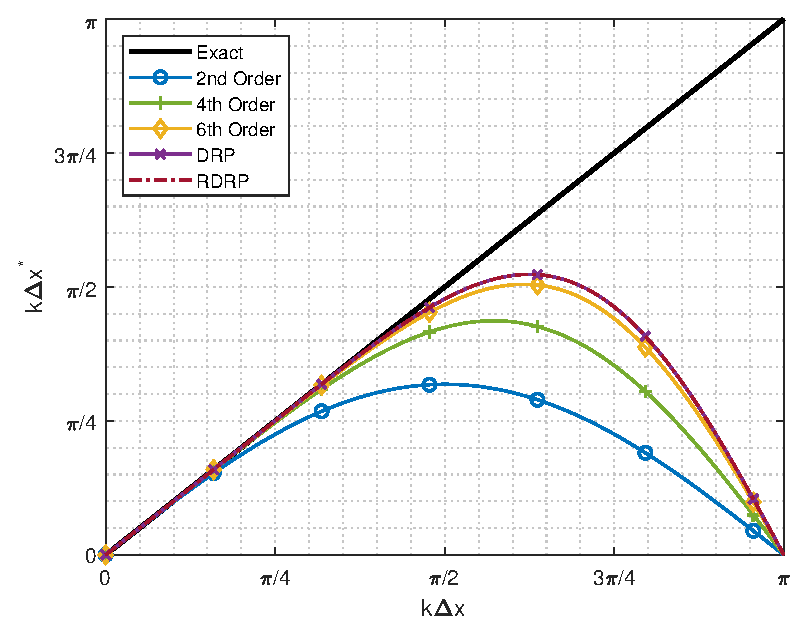
\includegraphics[width=0.7\textwidth]{Figures/Numerical_Wave.eps}
        \caption[Numerical wavenumber behavior] {Numerical Wavenumber Behavior of Standard Central Differencing Schemes. \label{fig:Num_wave}}
    \end{center}
\end{figure}


\begin{table}[hbtp!]
\caption[Maximum value of numerical wavenumber] {Maximum Value of Numerical Wavenumber for Spatial Differencing Methods}
\centering
\begin{tabular}{|c|c|}
\hline
{\textbf{Differencing Scheme}} & \textbf{Maximum $\mathbf{(k\Delta{x})^*}$} \\ \hline
{{Explicit 2nd Order}} & \textit{1.000} \\ \hline
{{Explicit 4th Order}} & \textit{1.400} \\ \hline
{{Explicit 6th Order}} & \textit{1.586} \\ \hline
{{Explicit DRP}} & \textit{1.664} \\ \hline
{{Explicit RDRP}} & \textit{1.664} \\ \hline
\end{tabular}
\\
\label{tab:Numerical_Wave}
\end{table}



In general, increasing the order of accuracy of a spatial differencing scheme will also improve its accuracy on a given grid. 
However, the stencil size of the scheme must be increased to obtain a higher order of accuracy, and these large-stencil schemes can have marginal stability near computational boundaries. 
An issue when using large stencil sizes for implicit time marching such as sixth order, Hixon's RDRP, or DRP schemes is that the matrix on the LHS is expensive to solve (due to the high number of diagonals). 

For instance, a three-point second-order central differencing stencil will result in a tridiagonal matrix on the LHS. 
The tridiagonal matrix is a sparse matrix with nonzero elements along the diagonal, first diagonal above, and first diagonal below the main diagonal. 
Most importantly, the Thomas Algorithm (a computationally efficient form of Gaussian elimination) can be used to solve the system of tridiagonal equations \cite{Thomas_Algo}. 
On the other hand, a heptadiagonal matrix (main diagonal with three diagonals above and below) is attained when using a seven-point stencil. 
Heptadiagonal matrices are much more computationally expensive to solve when compared to tridiagonal matrices. 

Taking advantage of Thomas's efficient algorithm, the left-hand side matrix of the seven-point stencil is replaced with an easier-to-solve matrix. 
In order to successfully replace such a matrix for an iterative steady-state solver, the time step stability must be studied. 

\subsubsection{Matrix Stability}
An eigenvalue analysis is used to test the numerical stability of a time step with different differencing stencil operators. 
Consider a periodic one-dimensional linear advection case discretized into $N$ equal intervals in space. 
A second order spatial difference is used on the LHS, and the governing equation is:

\begin{equation}
	\begin{split}
		\label{eq:LAE}
  			\left(I+\Delta{t}\cdot\left(\left.\frac{\partial}{\partial{x}}\right|_{LHS}\left(c\right)\right)\right)\Delta{u}~=&~-\Delta{t}\left(\left.\frac{\partial}{\partial{x}}\right|_{RHS}\left(c\right)\right) {u}_i^{n} \\
  			\Delta{u}+\frac{\nu}{2}\left(\Delta{u_{i+1}}-\Delta{u_{i-1}} \right)~=&~-\Delta{t}\left(\left.\frac{\partial}{\partial{x}}\right|_{RHS}\left(c\right)\right) {u}_i^{n} \\
  			\left[A\right]\left\{\Delta{u}\right\}~=&~\left[B\right]\left\{u_{i}^{n}\right\} \\
	\end{split}
\end{equation}
Where $[A]$ and $[B]$ are $N\times{N}$ (sparse) matrices and $\Delta{u},~u_{i}^{n}$ are $N$ vectors representing the value of the function at the nodes $x_i~=~i/N$.
Five different $RHS$ differencing stencils are tested in this publication:
%\begin{equation}
%	\begin{split}
%		\label{eq:Differencing Stencils}
%  			\left.\frac{\partial{f}}{\partial{x}}\right|_{i}~=&~\frac{f_{i+1}-f_{i-1}}{2\Delta{x}}~~\to~~\text{Second Order} \\
%  			\left.\frac{\partial{f}}{\partial{x}}\right|_{i}~=&~\frac{-f_{i+2}+8f_{i+1}-8f_{i-1}+f_{i-2}}{12\Delta{x}}~~\to~~\text{Fourth Order} \\
%  			\left.\frac{\partial{f}}{\partial{x}}\right|_{i}~=&~\frac{f_{i+3}-9f_{i+2}+45f_{i+1}-45f_{i-1}+9f_{i-2}-f_{i-3}}{60\Delta{x}}~~\to~~\text{Sixth Order} \\
%  			\left.\frac{\partial{f}}{\partial{x}}\right|_{i}~=&~\frac{f_{i+3}-8f_{i+2}+37f_{i+1}-37f_{i-1}+8f_{i-2}-f_{i-3}}{48\Delta{x}}~~\to~~\text{RDRP} \\
%	\end{split}
%\end{equation}
\begin{itemize}
	\item Second Order (E2):
		\begin{equation*}
			\left.\frac{\partial{f}}{\partial{x}}\right|_{i}~=~\frac{f_{i+1}-f_{i-1}}{2\Delta{x}}
		\end{equation*}
	\item Fourth Order (E4):
		\begin{equation*}
			\left.\frac{\partial{f}}{\partial{x}}\right|_{i}~=~\frac{-f_{i+2}+8f_{i+1}-8f_{i-1}+f_{i-2}}{12\Delta{x}}
		\end{equation*}	
	\item Sixth Order (E6):
		\begin{equation*}
			\left.\frac{\partial{f}}{\partial{x}}\right|_{i}~=~\frac{f_{i+3}-9f_{i+2}+45f_{i+1}-45f_{i-1}+9f_{i-2}-f_{i-3}}{60\Delta{x}}
		\end{equation*}
	\item RDRP \cite{RDRP}:
		\begin{equation*}
			\left.\frac{\partial{f}}{\partial{x}}\right|_{i}~=~\frac{f_{i+3}-8f_{i+2}+37f_{i+1}-37f_{i-1}+8f_{i-2}-f_{i-3}}{48\Delta{x}}
		\end{equation*}
	\item DRP \cite{DRP}:
		\begin{equation*}
			\left.\frac{\partial{f}}{\partial{x}}\right|_{i}~=~\frac{1}{\Delta{x}}
				\left(\begin{matrix} 	
					~~0.0208431427703f_{i+3} \\
					-~0.166705904415f_{i+2}  \\
					+~0.770882380518f_{i+1}  \\
					-~0.770882380518f_{i-1}  \\
					+~0.166705904415f_{i-2}  \\
					-~0.0208431427703f_{i-3}
				\end{matrix}
				\right)
		\end{equation*}
\end{itemize}
To analyze the stability of a time step we re-write Eq. (\ref{eq:LAE}) as:
\begin{equation}
\label{eq:AB}
	\begin{split}
  		[T]\{\Delta{u_i\}}~=&~[B]\{u_i^{n}\} \\
  		\left\{\frac{\Delta{u_i}}{u_i^{n}}\right\}~=&~[T]^{-1}[B] \\
  		\frac{u_i^{n+1}}{u_i^{n}} - [1]~=&~[T]^{-1}[B] \\
  		\frac{u_i^{n+1}}{u_i^{n}}~=&~[T]^{-1}[B] + [1] \\
  		~=&~[C]
	\end{split}
\end{equation}
The eigenvalues are calculated as:
\begin{equation}
	\begin{split}
		\label{eq:Magnitude_Of_Eigen}
  			\left|\frac{u_i^{n+1}}{u_i^{n}}\right|~=~\left|\lambda\left[C\right]\right|
	\end{split}
\end{equation}
If the magnitude of the eigenvalues is less than or equal to one, then the time step is stable.  
Otherwise, error terms will amplify, and the time step is unstable.
Note that matrices $[A]$ and $[B]$ are functions of the CFL:
\begin{equation}
	\begin{split}
		\label{eq:CFL}
  			\text{CFL}\to\nu~=~\frac{c\Delta{t}}{\Delta{x}}
	\end{split}
\end{equation}
Therefore the eigenvalues obtained are also functions of $\nu$. 

Figure \ref{fig:nu_vs_magnitude} shows the maximum magnitude of the eigenvalue (over 201 grid points) for the five different RHS stencils using periodic boundaries vs. $\nu$. 
As seen in the Figure, a second-order differencing stencil is stable. 
This is not a surprise since both LHS and RHS use the same differencing stencil. 
The stability under such conditions is shown to be less than one for any value of $\nu$ in Appendix \ref{Sec:Appendix:Stability_Fourier}.
The fourth-order difference was also stable when using periodic boundaries. 
This result is somewhat counterintuitive; however, a deeper analysis for the stability of fourth-order difference can be seen in Appendix \ref{sec:Appendix:Scaling_Fac}. 
Once the RHS spatial derivative changes to sixth, RDRP, or DRP, the time step is unstable regardless of the value of $\nu$. 


\begin{figure}[hbtp!]
	\centering
	{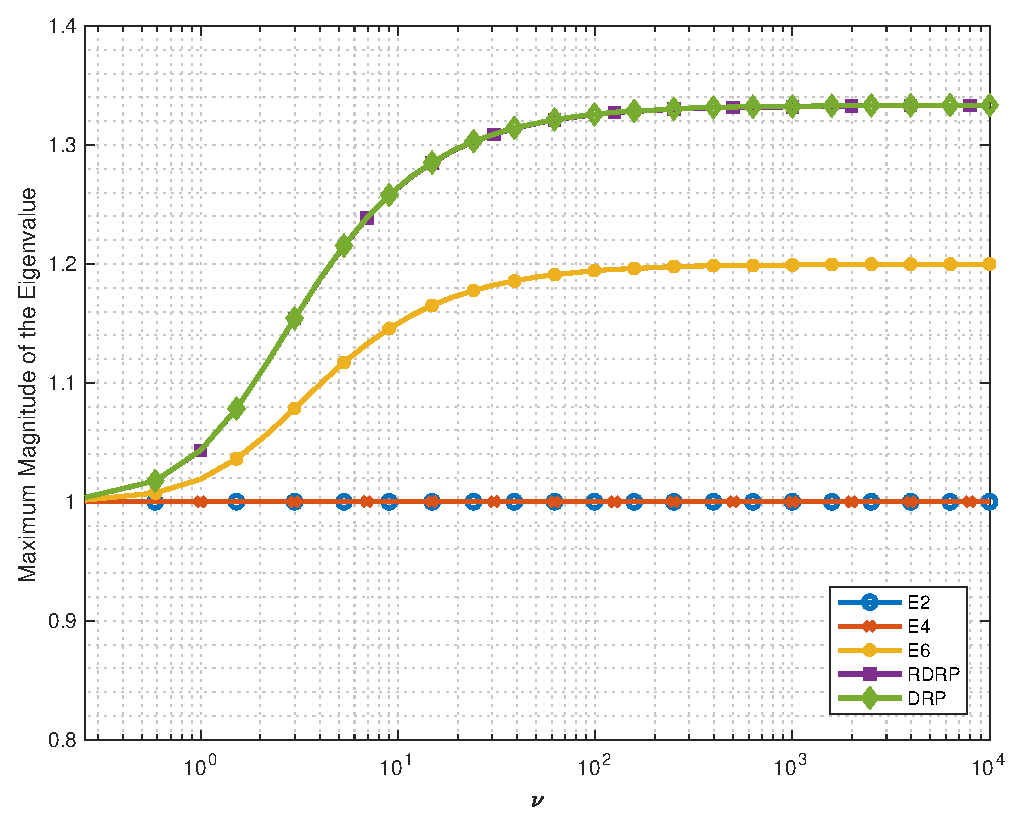
\includegraphics[width=0.7\textwidth]{Figures/nu_vs_magnitude}}
	\caption{Maximum Magnitude of the Eigenvalue vs $\nu$, 
	Periodic Tridiagonal Matrix LHS without Scaling Factors $\sigma$}
	\label{fig:nu_vs_magnitude}
\end{figure}
However, if Eq. (\ref{eq:LAE}) is modified to add a scaling factor $\sigma$ multiplying the spatial derivative on the LHS:
\begin{equation}
	\begin{split}
		\label{eq:LAE_Scaling}
  			\Delta{u}+\sigma\cdot\left(\frac{\nu}{2}\left(\Delta{u_{i+1}}-\Delta{u_{i-1}} \right)\right)~=&~-\Delta{t}\left(\left.\frac{\partial}{\partial{x}}\right|_{RHS}\left(c\right)\right) {u}_i^{n}
	\end{split}
\end{equation}
Can stability be obtained? If so, what are the values of the scaling factor $\sigma$? 

Through numerical testing, stability is obtained for all differencing stencils using periodic boundaries. 
Values of the periodic scaling factors are shown in Table \ref{tab:Scaling}; where Fig. \ref{fig:index_vs_mag_Scaling} highlights the magnitude of the eigenvalue vs. the number of grid points at a CFL of $\nu\to\infty$. 
%The eigendecomposition method to analyze stability helps study the maximum eigenvalues on the LHS and RHS. 
The periodic scaling factors ensure that the maximum eigenvalues from the second-order scheme (LHS) are greater than the maximum eigenvalues from the RHS schemes. 
Given that both spatial differencing use periodic boundaries, the numerical wavenumbers are knowns for all scheme. 
A detailed look on how to obtain the correct value for of the scaling factor $\sigma$ is shown in Appendix \ref{sec:Appendix:Scaling_Fac}. 
%\begin{figure}[hbtp!]
%	\centering
%	{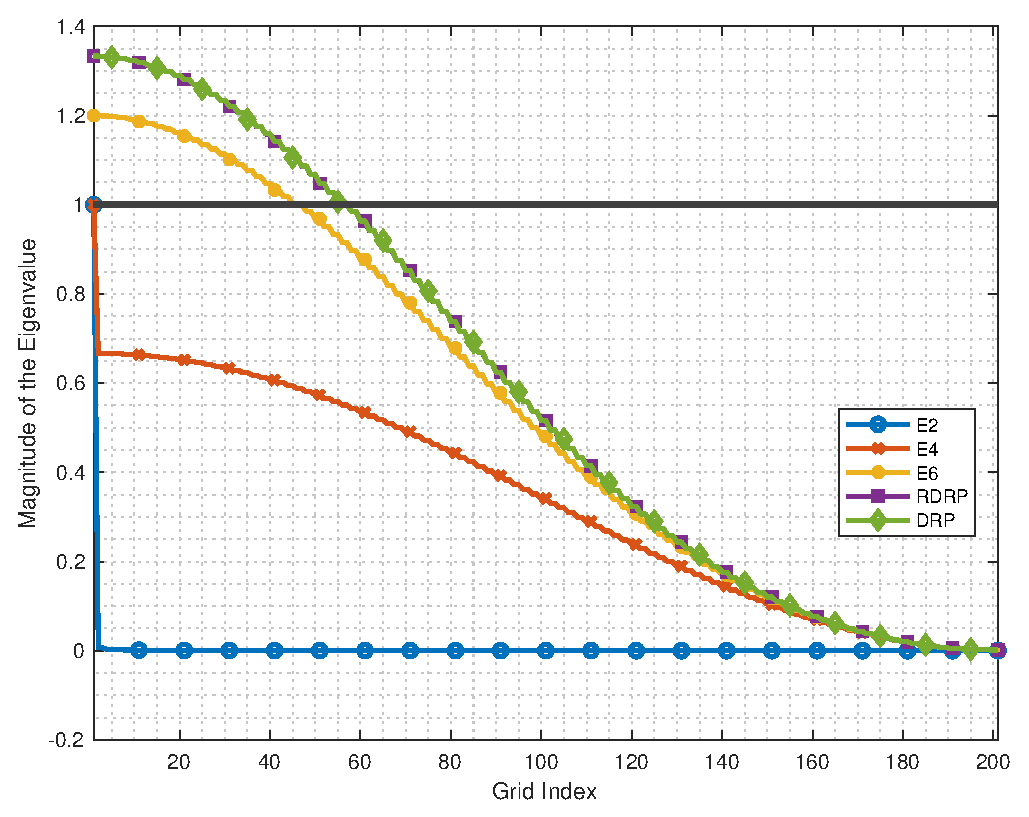
\includegraphics[width=0.7\textwidth]{Figures/index_vs_mag}}
%	\caption{Magnitude of Eigenvalue vs Grid Index  \\
%	Periodic tridiagonal matrix LHS without Scaling Factors $\sigma$, $\nu\to\infty$}
%	\label{fig:index_vs_mag}
%\end{figure}

\begin{figure}[hbtp!]
	\centering
	{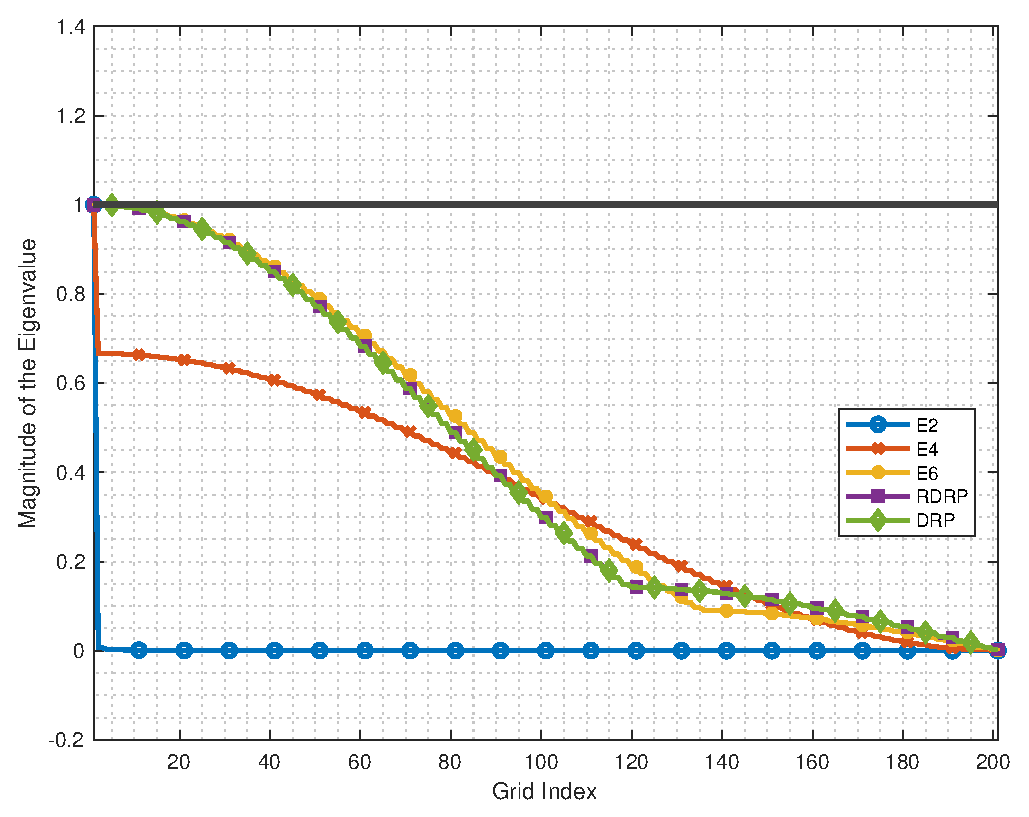
\includegraphics[width=.7\textwidth]{Figures/index_vs_mag_ScaleFactor_Periodic}}
	\caption{Magnitude of Eigenvalue vs Grid Index 
	Periodic Tridiagonal Matrix LHS with Scaling Factors $\sigma$, $\nu\to\infty$}
	\label{fig:index_vs_mag_Scaling}
\end{figure}

\subsubsection{Bounded Flow and Scaling Factors}
Before examining the benchmark problems and validating the periodic scaling factor values obtained, it is essential to compute the scaling factors with bounded flow.
For problems with periodic boundary conditions, the Fourier analysis presented above and in Appendix \ref{sec:Appendix:Scaling_Fac} may be used to assess the global errors and calculate periodic scaling factors. 
This, however, is not possible with other forms of boundary conditions such as a bounded flow. 
%Hence an eigendecomposition is once again needed to calculate the bounded scaling factors. 

For this analysis, all schemes use the Hixon et al. ''ghost point correction'' method, \cite{GPT, RDRP} in which the governing equations are directly solved at the boundary points. 
As described in the reference, the spatial derivatives are first computed for all directions, using the ''\textit{noBC}'' stencils in the direction normal to the boundary. 
A boundary conditions of:
\begin{equation}
	\begin{split}
		\label{eq:}
  			\left.\frac{\partial{f}}{\partial{x}}\right|_i^{BC}~=~0
	\end{split}
\end{equation}
is then applied as a ''correction'' to the normal derivative at the boundary, modifying the flux value at a nonphysical'' ghost point'' outside the computational domain.
This modified ghost point value affects the normal derivative at every grid point whose spatial derivative uses the ghost point value. 
These corrections are given in terms of the boundary normal derivative correction on the appropriate grid line in the reference \cite{GPT, RDRP}. 

%Using the eigendecomposition solver described in Section \ref{sec:Eigenvalue}, the bounded scaling factor was numerically calculated. 
%Once a value for the scaling factor was obtained on a given grid, the number of grid points used was varied in the eigendecomposition solver since the scaling factor asymptotes to a value.
%  
Values of the bounded scaling factors are calculated numerically and shown in Table \ref{tab:Scaling}; where Fig. \ref{fig:index_vs_mag_Scaling_Bounded} highlights the magnitude of the eigenvalue vs. the number of grid points at a CFL of $\nu\to\infty$. 


\begin{figure}[hbtp!]
	\centering
	{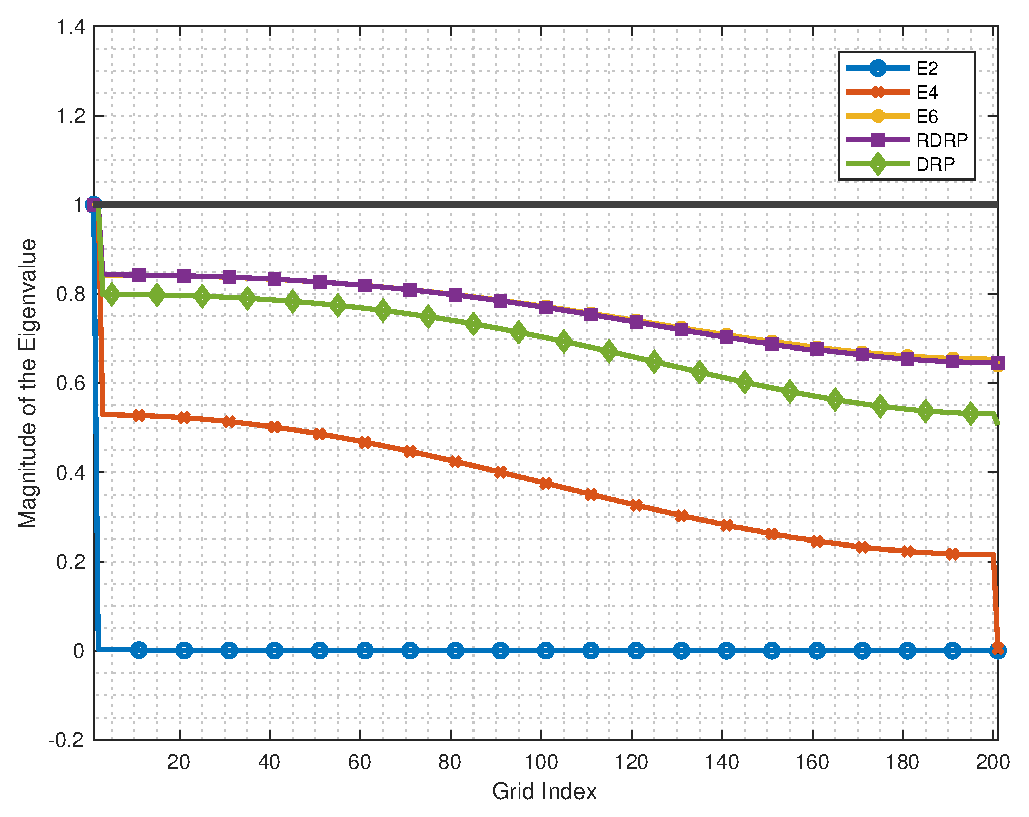
\includegraphics[width=.7\textwidth]{Figures/index_vs_mag_ScaleFactor_Bounded}}
	\caption{Magnitude of Eigenvalue vs Grid Index 
	Bounded tridiagonal matrix LHS with Scaling Factors $\sigma$, $\nu\to\infty$}
	\label{fig:index_vs_mag_Scaling_Bounded}
\end{figure}

\subsection{LU-SGS Stability}
\label{subsec:LUSGS}
Yoon and Jameson's LU-SGS numerical time step stability is analyzed in this section. The eigendecomposition setup explained in Section \ref{subsec:TriDi} is used again here.
Consider a periodic one dimensionsal linear advection case, that is discretized into $N$ equal intervals in space, the LU-SGS method is written as:
\begin{equation}
	\begin{split}
	\label{eq:LSGSU_LAE}
		LD^{-1}U\Delta{u}~=&~-\Delta{t}\left\{RHS\right\}^{n}_i
	\end{split}
\end{equation}
note that using the linear advection equation the jacobian of the flux, $A$, and the corresponding eigenvalue are:
\begin{equation}
	\begin{split}
		\label{eq:FluxJac_Eig}
  			A~=&~\frac{\partial{E}}{\partial{Q}}~=~c \\
  			\epsilon_A~=&~c
	\end{split}
\end{equation}
giving the decomposed positive and negative eigenvalues, $A^+$ and $A^-$ respectively:
\begin{equation}
	\begin{split}
		\label{eq:A_Plus_Minus}
  			A^{+}~=&~\frac{1}{2}\left(A+\epsilon_AI\right)~=~c \\
  			A^{-}~=&~\frac{1}{2}\left(A-\epsilon_AI\right)~=~0
	\end{split}
\end{equation}
thus:
\begin{equation}
	\label{eq:LDU}
	\begin{split}
            L~=&~I + \alpha\Delta{t}\left(D_x^-A^+\right)\\
		D~=&~I + \alpha\Delta{t}\left(A^+\right) \\
		U~=&~I + \alpha\Delta{t}\left(A^+\right)
	\end{split}
\end{equation}
where $D_x^-$ is a \textit{first order backward difference operator}:
\begin{equation}
	\begin{split}
		\label{eq:First_Order Difference}
  			D_x^-{A^+}~=&~
  			~=~\frac{{A}^{+}_{i}-{A}^{+}_{i-1}}{\Delta{x}}
	\end{split}
\end{equation}
To analyze the stability of a time step, re-write Eq. (\ref{eq:LSGSU_LAE}) as:
\begin{equation}
\label{eq:AB}
	\begin{split}
  		[L][D]^{-1}[U]\{\Delta{u_i\}}~=&~[B]\{u_i^{n}\} \\
  		[T]\{\Delta{u_i\}}~=&~[B]\{u_i^{n}\} \\
  		\frac{u_i^{n+1}}{u_i^{n}}~=&~[T]^{-1}[B] + [1] \\
  		~=&~[C]
	\end{split}
\end{equation}
The eigenvalues are calculated as:
\begin{equation}
	\begin{split}
		\label{eq:Magnitude_Of_Eigen}
  			\left|\frac{u_i^{n+1}}{u_i^{n}}\right|~=~\left|\lambda\left[C\right]\right|
	\end{split}
\end{equation}
If the magnitude of the eigenvalues is less than or equal to one, then the time step is stable.  
As seen in Fig. \ref{fig:LUSGS_index_vs_mag_Scaling_Bounded}, magnitudes of the eigenvalues are less than or equal to one as $\nu\to\infty$ without the need for periodic or bounded scaling factors. 
The most striking result to emerge from the data is that even with non-periodic boundaries, scaling factors are not needed when using the LU-SGS factorization on the LHS. 



\begin{figure}[hbtp!]
	\centering
	{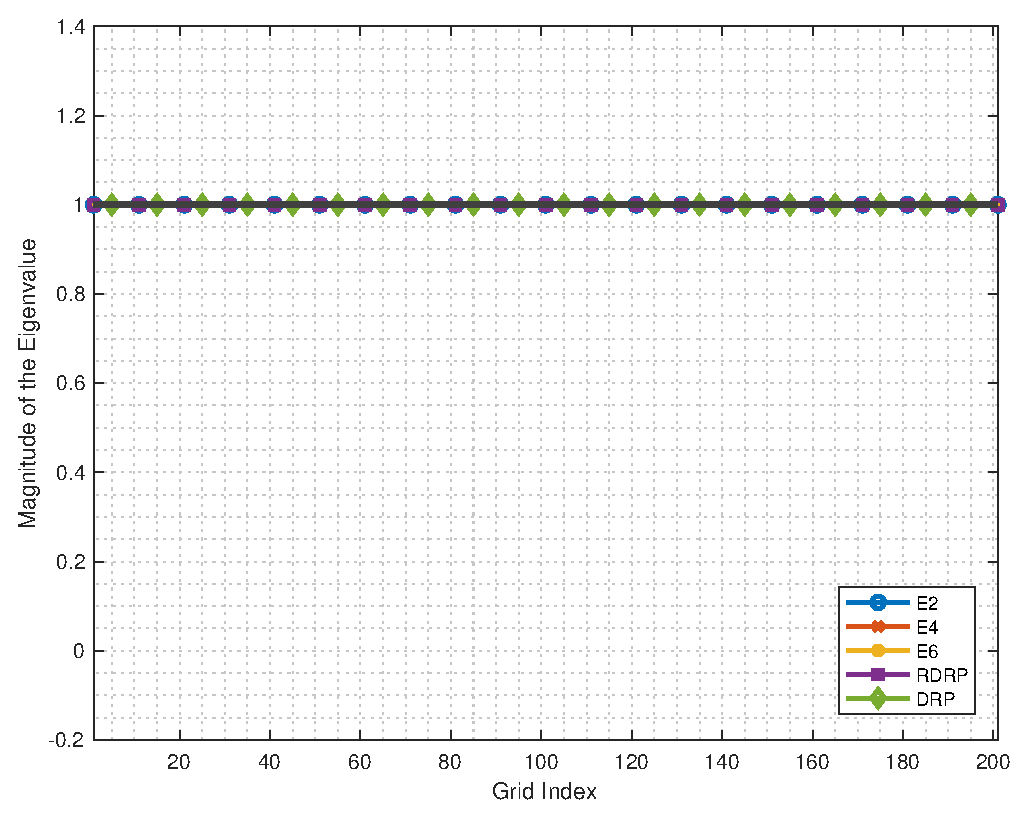
\includegraphics[width=.7\textwidth]{Figures/LUSGS_index_vs_mag_ScaleFactor_Periodic}}
	\caption{Magnitude of Eigenvalue vs Grid Index
	Bounded LU-SGS LHS, $\nu\to\infty$}
	\label{fig:LUSGS_index_vs_mag_Scaling_Bounded}
\end{figure}



\begin{table}[htp!]
\centering
\caption{Periodic and Bounded Flow Scaling Factors}
\begin{tabular}{|l|c|c|c|c|c|}
\hline
 & \multicolumn{1}{c|}{\textbf{$\sigma_{E2}$}} & \multicolumn{1}{c|}{\textbf{$\sigma_{E4}$}} & \multicolumn{1}{c|}{$\sigma_{E6}$} & \multicolumn{1}{c|}{$\sigma_{DRP}$} & \multicolumn{1}{c|}{$\sigma_{RDRP}$}\\ \hline
\textbf{Tridiagonal Matrix-Periodic} & \textit{1.0} & \textit{1.0} & \textit{$\nicefrac{11}{10}$} & \textit{1.166823618} & \textit{$\nicefrac{7}{6}$}\\ \hline
\textbf{LUSGS-Periodic} & \textit{1.0} & \textit{1.0} & \textit{1.0} & \textit{1.0} & \textit{1.0}\\ \hline
\textbf{Tridiagonal Matrix-Bounded} & \textit{1.0} & \textit{2.12179602298} & \textit{6.352796985} & 
	\textit{4.97487147161} & 
	\textit{6.36206870932}\\ \hline
\textbf{LUSGS-Bounded} & \textit{1.0} & \textit{1.0} & \textit{1.0} & 
	\textit{1.0} & 
	\textit{1.0}\\ \hline
\end{tabular}
\label{tab:Scaling}
\end{table}

\section{Numerical Results for Benchmark
Problems}
One way to analyze the stability of an implicit time step was shown in Section \ref{sec:Eigenvalue}; 
form the associated matrices using a finite number of points. Then use computer software to compute the eigenvalues, which then can be used to quantify the stability nature of each scheme. 
While this does provide at least a first-order measure of linear stability, the analysis is by no means rigorous or general. 
Hence, real-life nonlinear benchmark steady problems are studied in this section to validate the conclusions from the eigenvalue analysis. 

In Computational Fluid Dynamics and Computational Aeroacoustics, emphasis is given on calculating both the steady and unsteady flow. 
Various numerical schemes are developed to understand and predict noise generation and propagation physics correctly. 
To verify the correct implementation of those schemes and their performances, a range of validation problems with solutions are listed in the CAA Workshops \cite{CAA1, CAA2, CAA3}.

Two problems from the Third CAA workshop are studied in this paper: \textit{Category 1 Problem 1 and Category 1 Problem 2} \cite{CAA3}. 
Category 1 problems deal with internal propagation; 
the propagation of sound through a narrow passage with flow exists in many applications. 
Problem 1 models the upstream propagation of sound through a nozzle with near sonic conditions. 
For the second problem, a shock is present in the nozzle, making nonlinearities important. 


The Quasi-1D nonlinear Euler equations are used to solve these two problems. The equations are given in the conservative variables as:

\begin{equation}
    \label{eq:Euler}
    \frac{\partial{}}{\partial{t}} 
    \begin{Bmatrix}
        \rho \\
        \rho{u} \\
        E_{tot}
  \end{Bmatrix}+\frac{\partial{}}{\partial{x}}
    \begin{Bmatrix}
        \rho{u} \\
        \rho{u^2}+p \\
        u(E_{tot}+p)
  \end{Bmatrix} +\frac{1}{A}\frac{\partial{A}}{\partial{x}}
    \begin{Bmatrix}
        \rho{u} \\
        \rho{u^2} \\
        u(E_{tot}+p)
  \end{Bmatrix}= 0
\end{equation}
In these equations,
\begin{equation}
    \label{eq:Euler_pressure}
    \begin{split}
    p &= (\gamma-1)\Big(E_{tot}-\frac{\rho{u^2}}{2}\Big) \\
    \gamma &= 1.4
    \end{split}
\end{equation}
For the time-step, the CFL parameter $\nu$ is defined as:
\begin{equation}
	\begin{split}
		\label{eq:}
  			\nu_{physical}
  			~=&~\frac{\left(\left|u_i\right|+c_i\right)\Delta{t}}{\Delta{x}}\cdot\left(k\Delta{x}\right)^*
	\end{split}
\end{equation}
The area of the duct is given by:
\begin{equation}
	\begin{split}
		\label{eq:}
  			A(x)~=&~\left\{
  			\begin{matrix}
  				0.536572~-~0.198086e^{\left(-ln2\right)\left(\frac{x}{0.6}\right)^2} & x \geq 0 \\
  				1.0~-~0.661514e^{\left(-ln2\right)\left(\frac{x}{0.6}\right)^2} & x \leq 0
  			\end{matrix}
  			\right.
	\end{split}
\end{equation}
on a computational domain of $-10\leq~x~\leq10$. The duct area vs domain is shown in Fig. \ref{fig:Domain_Area}.

%The mean stagnation pressure and density are calculated as:
%\begin{equation}
%    \label{eq:Euler_BC_2}
%    \begin{split}
%    \overline{p_0}~= & ~\overline{p}\left(1+\frac{\gamma -1}{2}\overline{M}^2\right)^{\frac{\gamma}{\gamma-1}} \\
%    \overline{\rho_0}~= & ~\overline{\rho}\left(1+\frac{\gamma -1}{2}\overline{M}^2\right)^{\frac{1}{\gamma-1}} \\
%    \overline{M} ~ = & ~ \frac{\overline{u}}{\overline{c}} \\
%    \overline{c} ~ = & ~ \sqrt{\frac{\gamma{\overline{p}}}{\overline{\rho}}}
%    \end{split}
%\end{equation}
%mean flow conditions such as $\left(\overline{\rho},~\overline{u},~\overline{p} \right)$ are specified for each problem. 
%

The numerical solver for this work uses an implicit time marching scheme with
tridiagonal matrix and LU-SGS formulation on the LHS. 
The LHS spatial difference is coupled with scaling factors for stability. 
While the following spatial differences are used on the RHS:
\begin{itemize}
	\item Second Order (E2)
	\item Fourth Order (E4)
	\item Sixth Order (E6)
	\item RDRP  (RDRP)
\end{itemize}

In order to accurately predict the flow, it is crucial to apply the boundary conditions correctly; otherwise, the boundaries may (and will) generate spurious fluctuations and thereby contaminate the entire solution. 
Thompson's nonlinear boundary conditions are used (referred to as characteristic boundaries in the literature).  
The Thompson approach \cite{Thompson1, Thompson2} uses an eigendecomposition on the Euler flux Jacobian matrix to generate the eigenvalues and eigenvector matrices, which are then used to diagonalize and decompose the equations. 
This decomposition generates three equations, when compared to the linear advection equation, can classify three different waves:
\begin{enumerate}
	\item An entropy wave, convecting with the flow:
		\begin{equation*}
			\frac{\partial{A_s}}{\partial{t}}~=~p_t-c^2\rho_t
		\end{equation*}
	\item A downstream-running acoustic wave, convecting with the flow and propagating downstream at the speed of sound:
		\begin{equation*}
			\frac{\partial{A_+}}{\partial{t}}~=~p_t+\rho{c}u_t
		\end{equation*}
	\item An upstream-running acoustic wave, convecting with the flow and propagating upstream at the speed of sound:
		\begin{equation*}
			\frac{\partial{A_-}}{\partial{t}}~=~p_t-\rho{c}u_t
		\end{equation*}
\end{enumerate}
Following Thompson's approach, waves leaving the domain are left unspecified. 
The calculations of such waves are determined using a one-sided difference. 
Waves that are entering the domain must be specified.

For both Category 1 problems, the inflow and outflow boundaries are subsonic. 
An entropy and downstream running acoustic waves are specified using the mean stagnation pressure and mean stagnation density for the inflow boundary.
The outflow boundary specifies the upstream-running acoustic wave using the mean exit pressure. 

\begin{figure}[hbtp!]
	\centering
{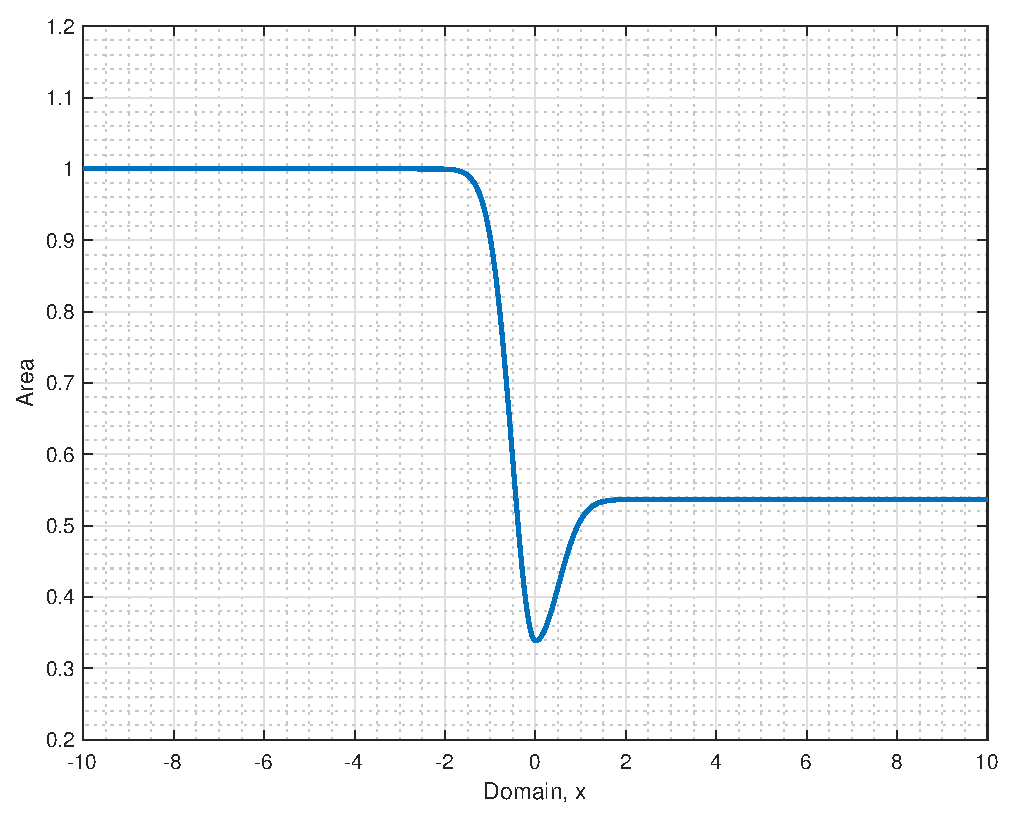
\includegraphics[width=0.7\textwidth]{Figures/Area}}
  	\caption{Category 1 Problems Domain vs Area}
  	\label{fig:Domain_Area}
\end{figure}
 
\subsection{Category 1 Problem 1: Propagation of Sound Waves through a Transonic Nozzle}

The problem is the upstream propagation of an acoustic wave through a transonic, nearly choked nozzle flow. 
The mean flow is set as:
\begin{equation*}
	\left\{
	\begin{matrix}
		\overline{\rho} \\
		\overline{u} \\
		\overline{p}
	\end{matrix}
	\right\}~=~
	\left\{
	\begin{matrix}
		1.0 \\
		0.4 \\
		\frac{1}{\gamma}
	\end{matrix}
	\right\}
\end{equation*}
An explicit tenth-order Kennedy and Carpenter's artificial dissipation operator that provides damping for the inviscid nonlinear calculations is added to the equation \cite{Kennedy_Carpt}. The initial condition is set to the mean flow values to solve the steady mean distribution. 

In this test case, an inviscid flow travels through a converging-diverging nozzle. 
This is a fully subsonic flow since there is no discontinuity in pressure.
A pressure drop is expected as the flow accelerates through the throat and then rises again as the flow backs down in Fig. \ref{fig:LUSGS_C1P1} and Fig. \ref{fig:TriDi_C1P1}. 
Both tridiagonal matrix bounded scaling factors and LU-SGS LHS formulation agrees well with the exact solution. 
The convergence of each scheme was determined by calculating the residual of the fluxes. 
Figure \ref{fig:LUSGS_C1P1_ROC} and \ref{fig:TriDi_C1P1_ROC} shows the residual vs iteration for the schemes. 
The Figures indicate converged solutions for the various RHS difference formulation. 
A value of $\Delta{t}\to\infty$ is set such that the LHS schemes reduce to a Newton iteration. 
However, the unsteady results are calculated to highlight the effect of higher-order difference stencils.  

Once the steady mean-flow results are obtained, the upstream propagating perturbation starts at the boundary, and the unsteady results are studied.  
Here, a small amplitude acoustic wave is generated way downstream and propagate upstream through the narrow passage of the nozzle throat:
\begin{equation*}
	\left\{
	\begin{matrix}
		{\rho}' \\
		{u}' \\
		{p}'
	\end{matrix}
	\right\}_{outflow}~=~
\epsilon
	\left\{
	\begin{matrix}
		1 \\
		-1 \\
		1
	\end{matrix}
	\right\}\cos\left[\omega\left(\frac{x_{outflow}}{1-M_{outflow}}+t\right)\right]
\end{equation*}
where $\epsilon=10^{-5}$ and $\omega=0.6\pi$. The inflow boundaries are set to:
\begin{equation*}
	\begin{split}
		\label{eq:}
  			\left.\frac{\partial{A_s}}{\partial{t}}\right|_{inflow}~=&~0 \\
  			\left.\frac{\partial{A_+}}{\partial{t}}\right|_{inflow}~=&~0
	\end{split}
\end{equation*}
where the outflow is:
\begin{equation*}
	\left.\frac{\partial{A_-}}{\partial{t}}\right|_{outflow}~=~
		-2\epsilon\omega\cdot{\sin}\left[\omega\left(\frac{10}{1-0.4} +t\right) \right]
\end{equation*}
%
%Initially, the problem was run with a uniformly-spaced grid to determine the necessary spacing at $x=0$ (the nozzle throat). 
%This was obtained at 1351 equally-spaced points, or a $\Delta{x}$ of 0.0148. 
%The minimum spacing was then set, and the grids were stretched to a maximum $\Delta{x}$ of 0.148 and were uniform to the boundary. 
%%The stretched grid solutions were then compared with the exact solution for accuracy. 
%Figure \ref{fig:Domain_Deltax} shows the grid spacing distribution as a function of x. 

Figure \ref{fig:Unsteady_C1P1} show the pressure perturbation using tridiagonal matrix and LU-SGS LHS formulation, along with low and high order RHS differencing stencils. 
The unsteady solution is taken once a periodic steady state is reached, uses 46 steps per cycle. An optimized $2^{nd}$ order optimized backward difference formulation \cite{HixonImplicit} is used to approximate the time derivative:
\begin{equation}
	\begin{split}
		\label{eq:2ndOrderdQdT}
  			\left.\frac{\partial{Q}}{\partial{t}}\right|_i~=&~\frac{10Q_i^{n+1, k}-15Q_i^n+6Q_i^{n-1}-Q_i^{n-2}}{6\Delta{t}}
	\end{split}
\end{equation}
The CFL is calculated as:
\begin{equation*}
	\nu_{physical}
  			~=~\frac{\left(\left|u_i\right|+c_i\right)}{\Delta{x}}\cdot\left(\frac{2\pi}{\omega}\cdot\frac{1}{\cdot Steps~Per~Cycle}\right)\cdot\left(k\Delta{x}\right)^*
\end{equation*}


It is seen that second-order spatial difference cannot accurately predict the pressure perturbation where the higher-order scheme, RDRP, agrees well with the exact. 
The value of $\nu_{physical}$ for each test-case is shown in Table \ref{tab:C1P1}.   


\begin{figure}[hbtp!]
	\centering
	{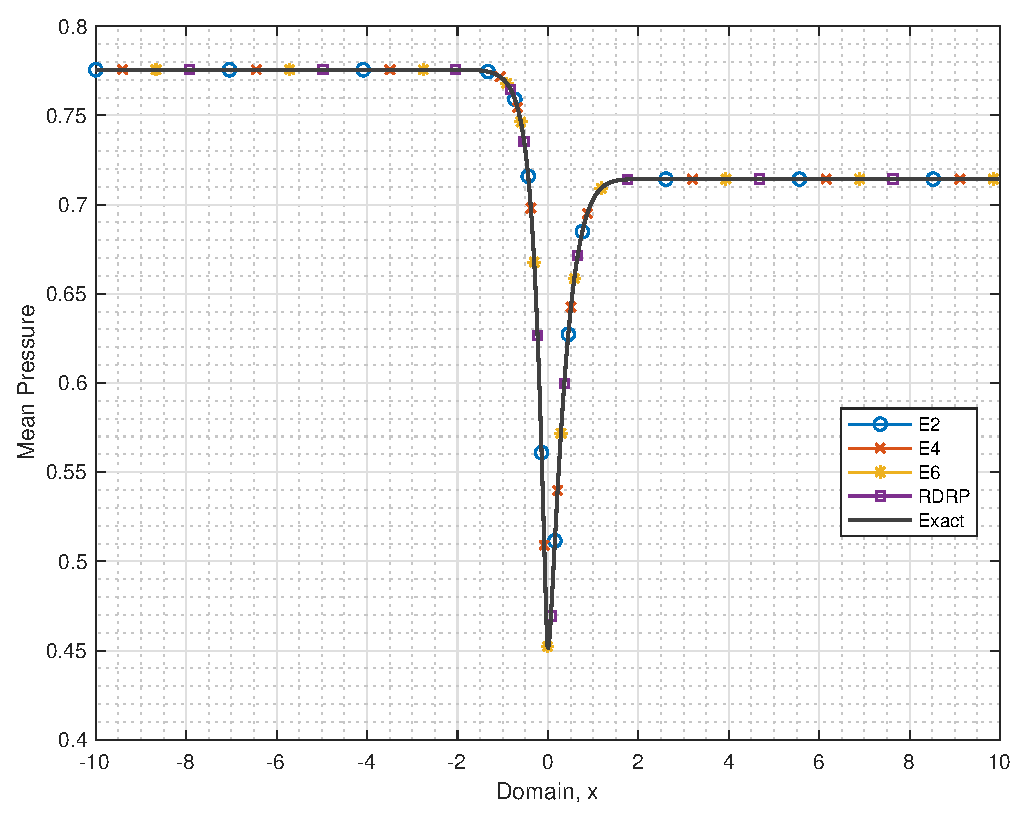
\includegraphics[width=.7\textwidth]{Figures/LUSGS_C1P1}}
	\caption{Domain vs Mean Pressure for Category 1 Problem 1, LU-SGS LHS}
	\label{fig:LUSGS_C1P1}
\end{figure}

\begin{figure}[hbtp!]
	\centering
	{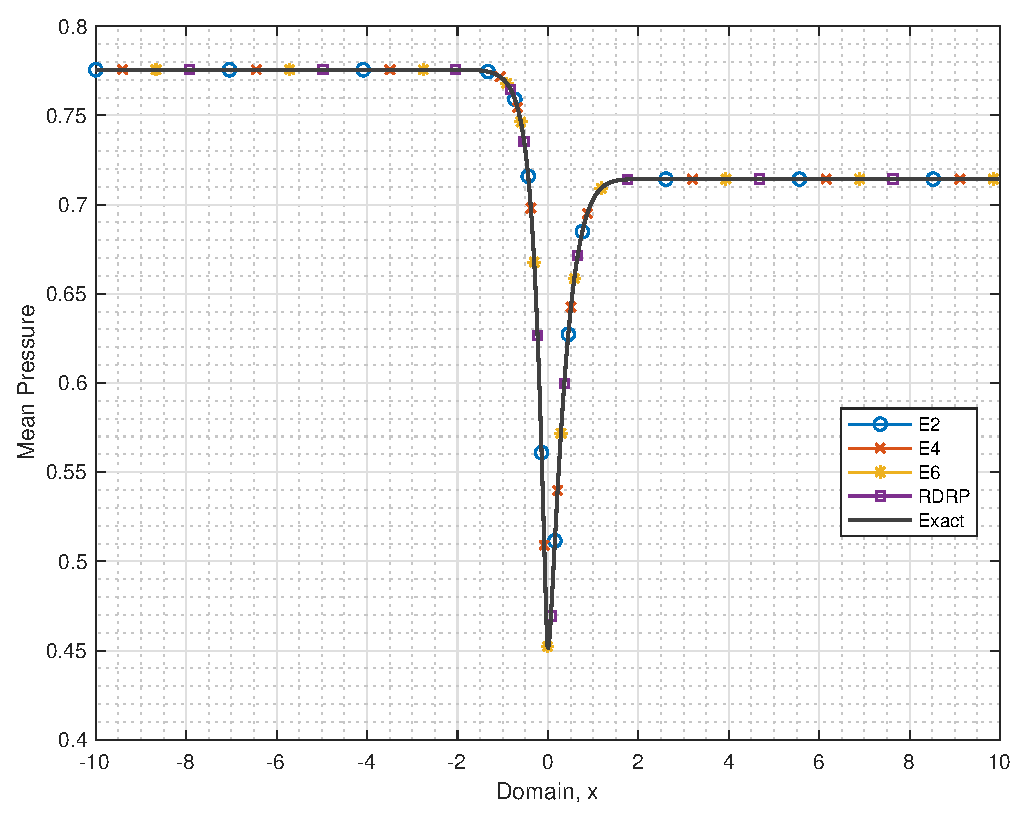
\includegraphics[width=.7\textwidth]{Figures/TriDi_C1P1}}
	\caption{Domain vs Mean Pressure for Category 1 Problem 1, tridiagonal matrix LHS}
	\label{fig:TriDi_C1P1}
\end{figure}


\begin{figure}[hbtp!]
	\centering
	{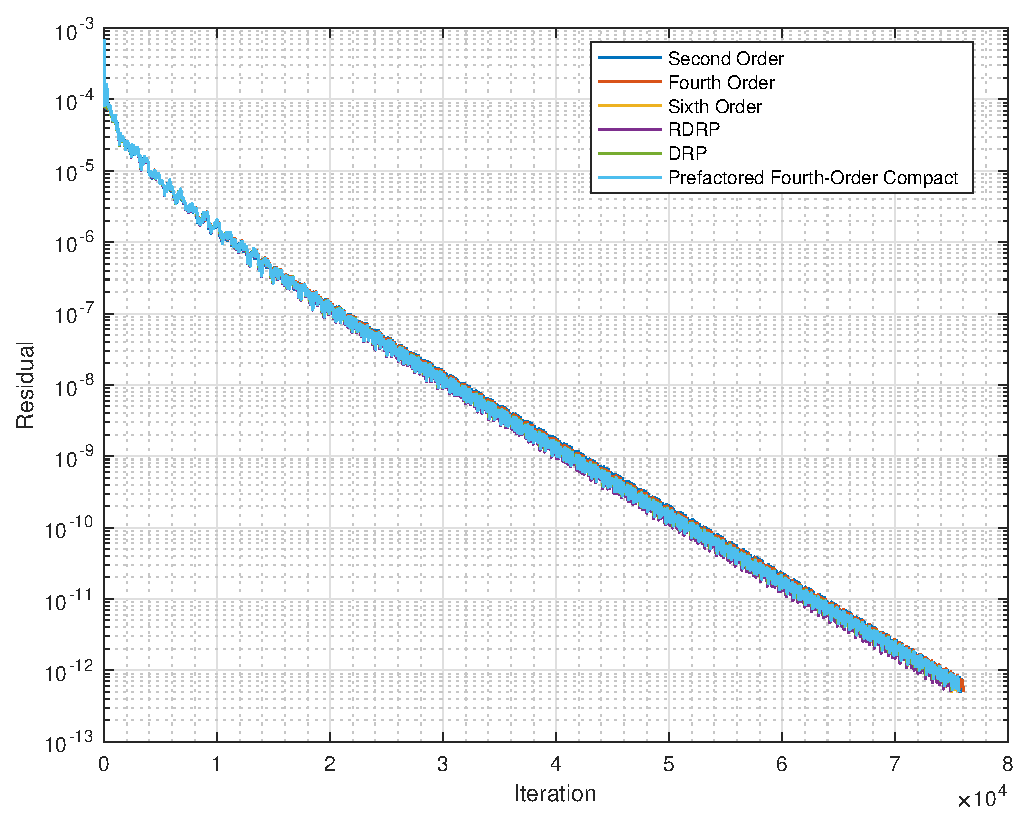
\includegraphics[width=.7\textwidth]{Figures/C1P1_LUSGS_ROC}}
	\caption{Residual vs Iteration Category 1 Problem 1, LU-SGS LHS}
	\label{fig:LUSGS_C1P1_ROC}
\end{figure}

\begin{figure}[hbtp!]
	\centering
	{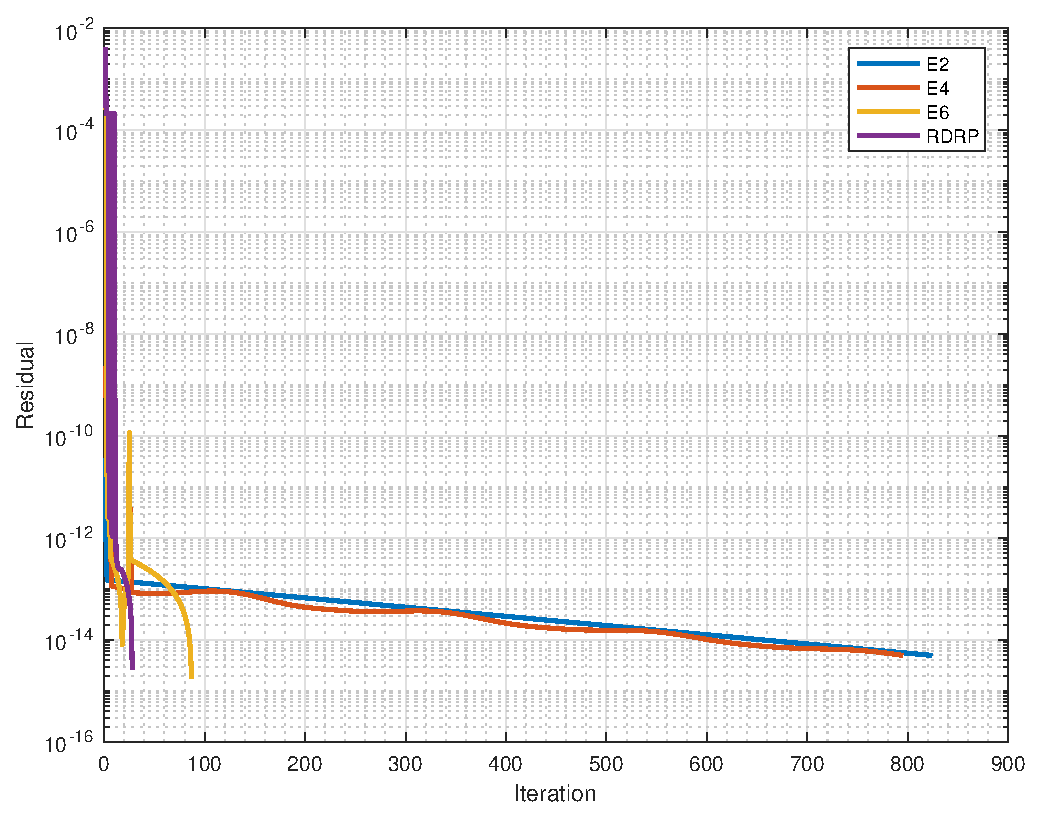
\includegraphics[width=.7\textwidth]{Figures/C1P1_TriDi_ROC}}
	\caption{Residual vs Iteration Category 1 Problem 1, Tridiagonal Matrix LHS}
	\label{fig:TriDi_C1P1_ROC}
\end{figure}

\begin{figure}[hbtp!]
	\centering
	{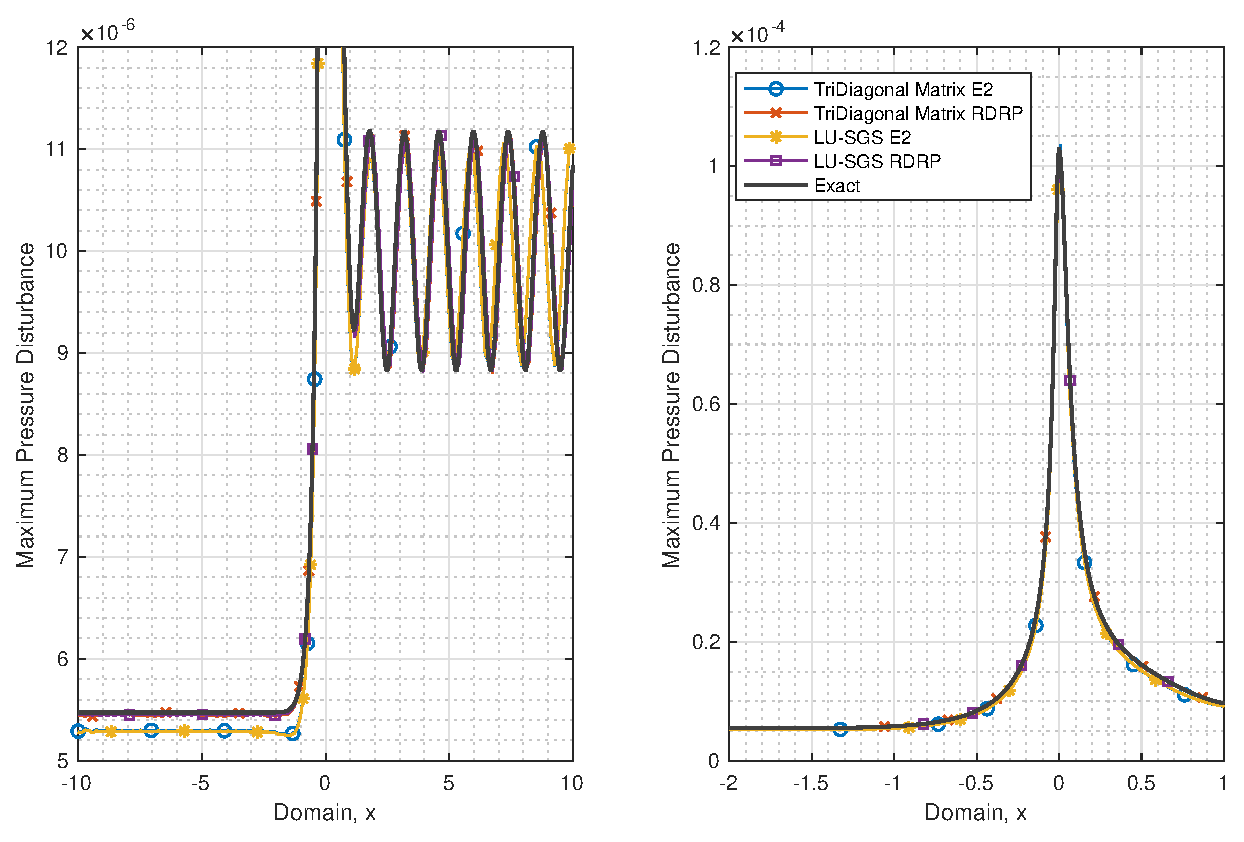
\includegraphics[width=1.0\textwidth]{Figures/Max_Dis_Closeup_Both}}
	\caption{Maximum Pressure Disturbance for Category 1 Problem 1}
	\label{fig:Unsteady_C1P1}
\end{figure}


\begin{table}[htp!]
\centering
\caption{CFL Value for Each Scheme, Category 1 Problem 1}
\label{tab:C1P1}
\begin{tabular}{|c|c|c|}
\hline
\textbf{LHS Formulation} & \textbf{RHS Differencing Stencil} & \textbf{$\boldsymbol{\nu_{physical}}$} \\ \hline
\textit{Tridiagonal Matrix} & \textit{E2}   & \textit{8.90446} \\ \hline
\textit{Tridiagonal Matrix} & \textit{RDRP} & \textit{14.8145} \\ \hline
\textit{LU-SGS}             & \textit{E2}   & \textit{8.90514} \\ \hline
\textit{LU-SGS}             & \textit{RDRP} & \textit{14.8163} \\ \hline
\end{tabular}
\end{table}

\subsection{Category 1 Problem 2: Shock-Sound Interaction}

The problem is the upstream propagation of an acoustic wave through a shock wave in a convergent-divergent nozzle. 
The mean flow is set as:
\begin{equation*}
	\left\{
	\begin{matrix}
		\overline{\rho} \\
		\overline{u} \\
		\overline{p}
	\end{matrix}
	\right\}~=~
	\left\{
	\begin{matrix}
		1.0 \\
		0.2006533 \\
		\frac{1}{\gamma}
	\end{matrix}
	\right\}
\end{equation*}
At the outflow boundary, the pressure is set such that it creates a shock: 
\begin{equation*}
	p_{exit}~=~0.6071752
\end{equation*}
The initial condition is set to the mean flow values to solve the steady mean distribution. 

This is a flow with a supersonic region and a shock downstream of the throat. 
The existence of a shock can be seen in a steep increase in pressure in Fig. \ref{fig:LUSGS_C1P2} and Fig. \ref{fig:TriDi_C1P2}. 
The shock is a discontinuity in the flow, which can cause oscillation in the solutions. 
Note, however, that the shock strength and location are consistent with all differencing stencils regardless of the LHS formulation.  
Both tridiagonal matrix bounded scaling factors and LU-SGS LHS formulation agrees well with the exact solution. 
The convergence of each scheme was determined by calculating the residual of the fluxes. 
Figure \ref{fig:LUSGS_C1P2_ROC} shows the residual vs. iteration, indicating converged solutions for the various RHS difference formulation. 
A value of $\Delta{t}\to\infty$ is set such that the LHS schemes reduce to a Newton iteration.   

Once the steady mean-flow results are obtained, the downstream propagating perturbation starts at the boundary, and the unsteady results are studied.  
Here, a small amplitude acoustic wave is generated upstream and propagate downstream through the narrow passage of the nozzle throat:
\begin{equation*}
	\left\{
	\begin{matrix}
		{\rho}' \\
		{u}' \\
		{p}'
	\end{matrix}
	\right\}_{inflow}~=~
\epsilon
	\left\{
	\begin{matrix}
		1 \\
		1 \\
		1
	\end{matrix}
	\right\}\sin\left[\omega\left(\frac{x_{inflow}}{1+M_{inflow}}-t\right)\right]
\end{equation*}
where $\epsilon=10^{-5}$ and $\omega=0.6\pi$.  
The inflow boundary is set to:
\begin{equation*}
	\begin{split}
		\left.\frac{\partial{A_s}}{\partial{t}}\right|_{inflow}~=&~0 \\
		\left.\frac{\partial{A_+}}{\partial{t}}\right|_{inflow}~=&~-2\epsilon\omega cos\left[\omega\left(\frac{x_{inflow}}{1 + M_{inflow}}-t \right)\right]
	\end{split}
\end{equation*}
where the outflow is:
\begin{equation*}
		\left.\frac{\partial{A_-}}{\partial{t}}\right|_{outflow}~=~0
\end{equation*}

Figures \ref{fig:Unsteady_C1P2} and \ref{fig:Exit_C1P2} show the instantaneous pressure perturbation vs. domain and exit pressure vs. time, respectively. 
Both results use tridiagonal matrix and LU-SGS LHS formulation, along with low and high order RHS differencing stencils. 
It is seen that second-order spatial difference cannot accurately predict the pressure perturbation where the higher-order scheme, RDRP, agrees well with the exact. 
The value of $\nu_{physical}$ for each test-case is shown in Table \ref{tab:C1P2}.   

\begin{figure}[hbtp!]
	\centering
	{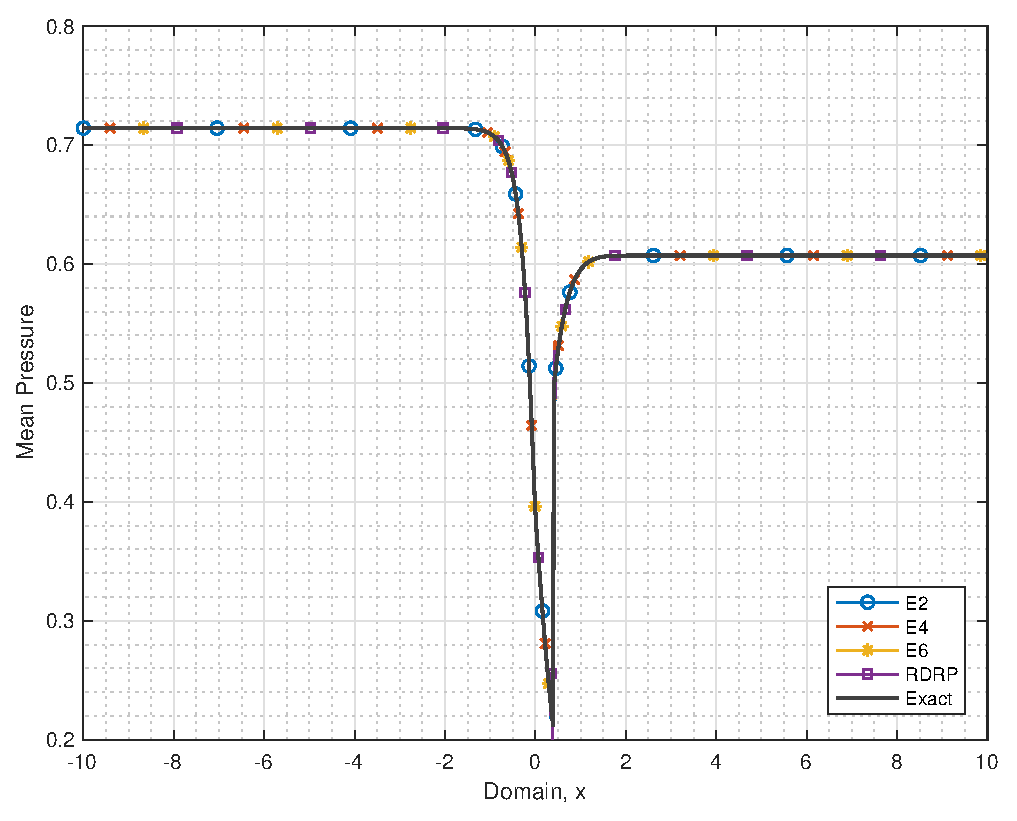
\includegraphics[width=.7\textwidth]{Figures/LUSGS_C1P2}}
	\caption{Domain vs Mean Pressure for Category 1 Problem 2, LU-SGS LHS}
	\label{fig:LUSGS_C1P2}
\end{figure}

\begin{figure}[hbtp!]
	\centering
	{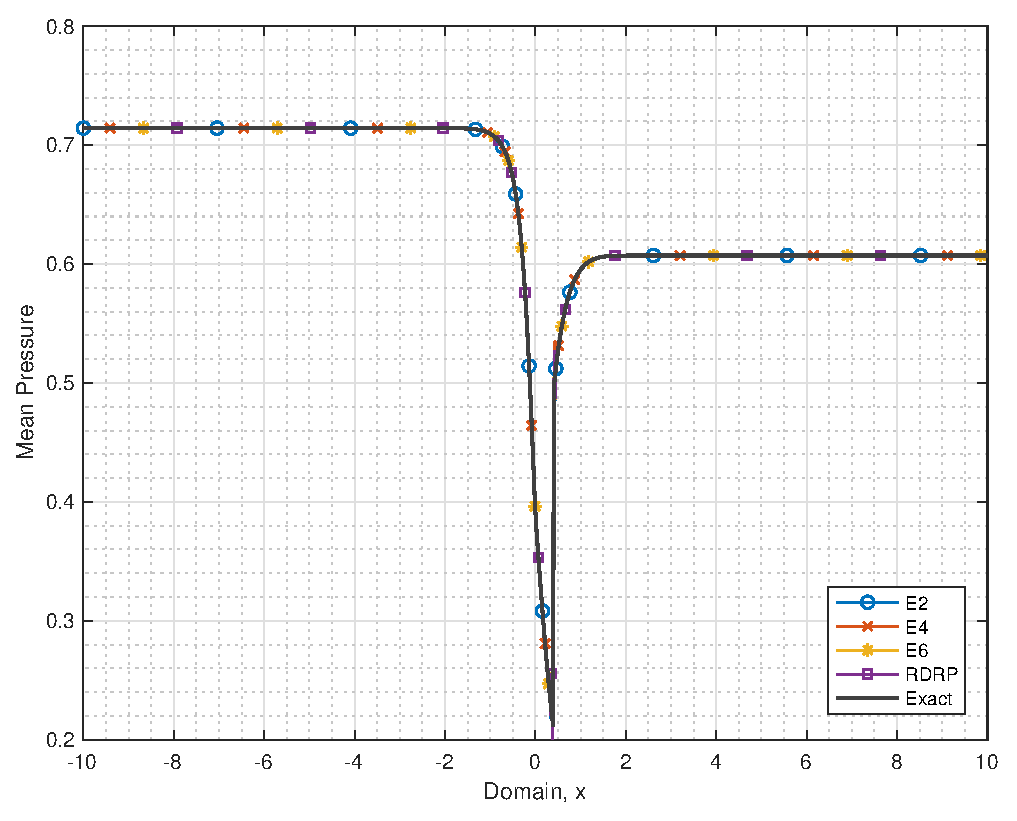
\includegraphics[width=.7\textwidth]{Figures/TriDi_C1P2}}
	\caption{Domain vs Mean Pressure for Category 1 Problem 2, tridiagonal matrix LHS}
	\label{fig:TriDi_C1P2}
\end{figure}

\begin{figure}[hbtp!]
	\centering
	{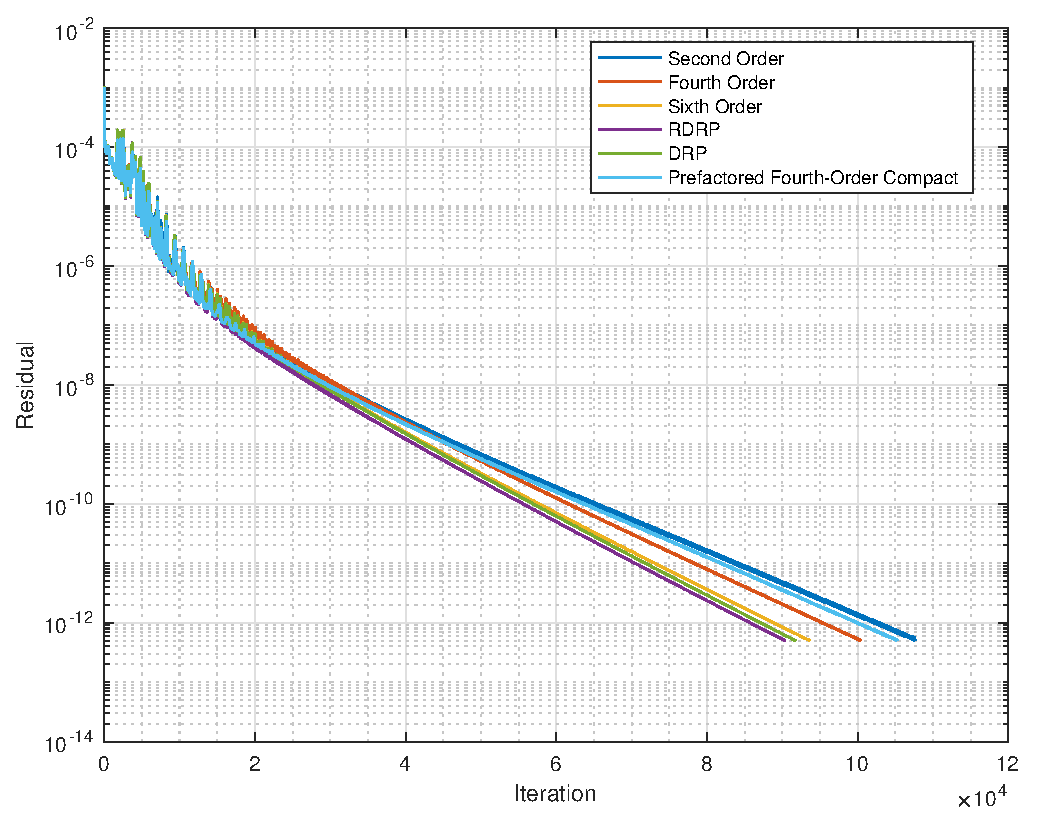
\includegraphics[width=.7\textwidth]{Figures/C1P2_LUSGS_ROC}}
	\caption{Residual vs Iteration Category 1 Problem 2, LU-SGS LHS}
	\label{fig:LUSGS_C1P2_ROC}
\end{figure}

\begin{figure}[hbtp!]
	\centering
	{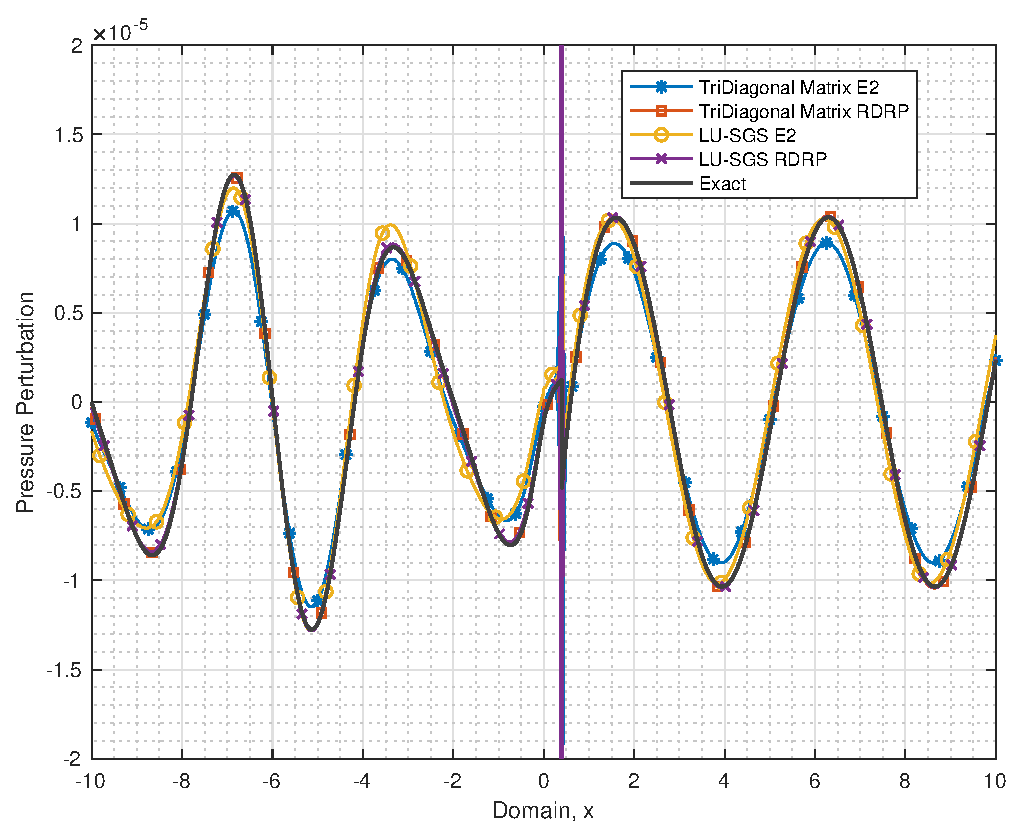
\includegraphics[width=0.7\textwidth]{Figures/Instantaneous_C1P2}}
	\caption{Perturbation Pressure Distribution for Category 1 Problem 2}
	\label{fig:Unsteady_C1P2}
\end{figure}



\begin{figure}[hbtp!]
	\centering
	{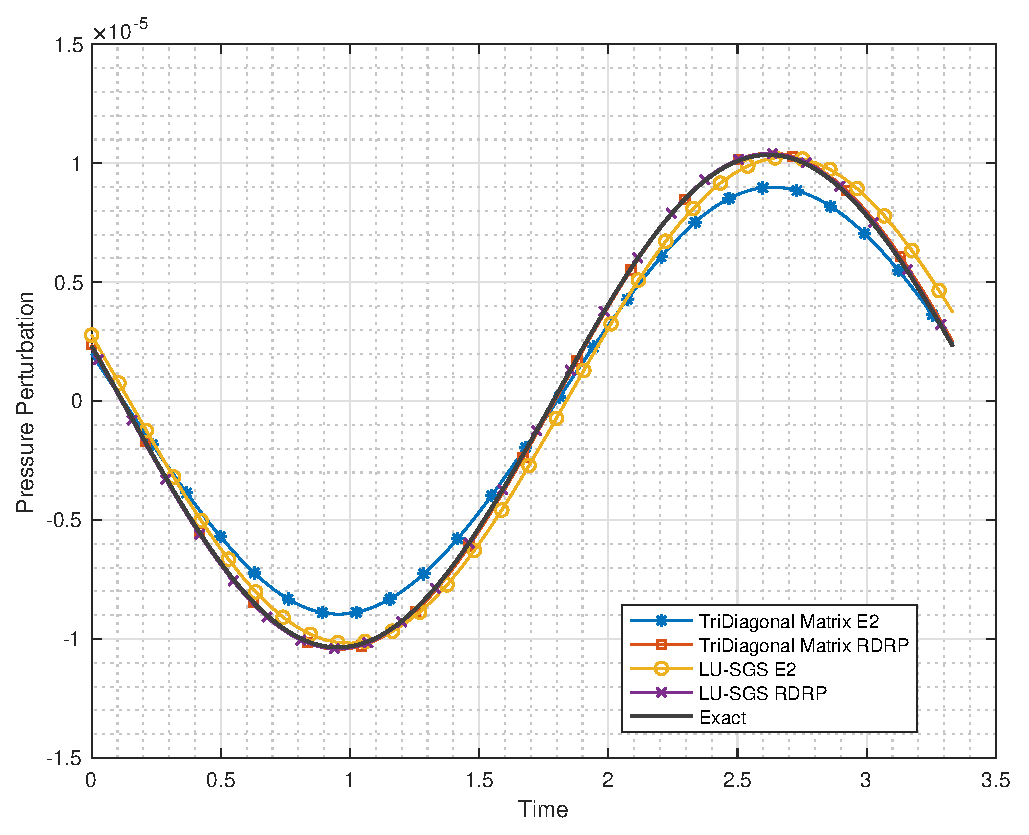
\includegraphics[width=0.7\textwidth]{Figures/Exit_vs_Time}}
	\caption{Perturbation Pressure History at Exit Plane, Category 1 Problem 2}
	\label{fig:Exit_C1P2}
\end{figure}


\begin{table}[htp!]
\centering
\caption{CFL Value for Each Scheme, Category 1 Problem 2}
\label{tab:C1P2}
\begin{tabular}{|c|c|c|}
\hline
\textbf{LHS Formulation} & \textbf{RHS Differencing Stencil} & \textbf{$\boldsymbol{\nu_{physical}}$} \\ \hline
\textit{Tridiagonal Matrix} & \textit{E2}   & \textit{10.7218} \\ \hline
\textit{Tridiagonal Matrix} & \textit{RDRP} & \textit{17.8411} \\ \hline
\textit{LU-SGS}             & \textit{E2}   & \textit{10.7221} \\ \hline
\textit{LU-SGS}             & \textit{RDRP} & \textit{17.8415} \\ \hline
\end{tabular}
\end{table}

\section{Conclusion}
The present research aimed to establish a highly efficient implicit solver while using higher-order spatial differencing schemes. 
Through the use of scaling factors, the LHS matrix was replaced with an easier to solve matrix hence cutting down on the computational work needed for the iterative steady-state solver. 
Although the current study is based on one-dimensional problems, the findings suggest stability is possible for tridiagonal matrix formulation if scaling factors are used on the LHS spatial difference. 
Scaling factors ensured that the maximum eigenvalues from the LHS spatial difference were greater than the RHS.  
Different boundaries would yield different scaling factor values. 
The second significant finding in this work was, LU-SGS formulation on the LHS does not require scaling factors regardless of the boundaries used. 
Both Tri-Di and LU-SGS formulation were tested against CAA workshop data; the numerical solution agrees well with the exact.  

Due to factorizations in two and three dimensions, new error terms are introduced when dealing with ADI. 
Hence, testing the scaling factors in multiple dimensions would be fruitful for further work. 
Further research might also explore if scaling factors are needed with compact differencing schemes and also validating viscous flow solutions. 

\section{Appendix}
\subsection{Stability of an Implicit Scheme}
{
{\label{Sec:Appendix:Stability_Fourier}
To investigate the stability of an implicit time step, the linearized inviscid one dimensional linear advection equation is used, which is written as:
\begin{equation}
	\begin{split}
		\label{eq:LAE_Simple_Version}
  			u_t+cu_x~=~0
	\end{split}
\end{equation}
Using a the Second Order (E2) central differencing scheme for spatial differencing, combined with an implicit first order time marching scheme, the discretized equation on a uniform grid with spacing $\Delta{x}$ is:
\begin{equation}
	\begin{split}
		\label{eq:LAE_RDRP}
  			\Delta{u_i}+\frac{\nu}{2}\left(\Delta{u_{i+1}}-\Delta{u_{i-1}}\right) ~=&~-\frac{\nu}{2}\left(u^n_{i+1}-u^n_{i-1}\right)
	\end{split}
\end{equation}
where
\begin{equation*}
	\nu~=~\frac{c\Delta{t}}{\Delta{x}}
\end{equation*}
The truncation error is defined as:
\begin{equation*}
	u_i^n~=~D_i^n+\epsilon_i^n
\end{equation*}
where $D$ exactly satisfies the discretized equation. Substituting in and eliminating $D$ gives the error equation as:
\begin{equation}
	\begin{split}
		\label{eq:Error_Equation}
  			\Delta{\epsilon_i}+\frac{\nu}{2}\left(\Delta{\epsilon_{i+1}}-\Delta{\epsilon_{i-1}}\right) ~=&~-\frac{\nu}{2}\left(\epsilon^n_{i+1}-\epsilon^n_{i-1}\right)
	\end{split}
\end{equation}
Assuming that the error is a linear combination of Fourier modes in space: 
\begin{equation}
	\begin{split}
		\label{eq:Error_Fourier}
  			\epsilon^n~=&~\sum_{k=-\frac{\pi}{\Delta{x}}}^{\frac{\pi}{\Delta{x}}}{A_k^n e^{ikx}} \\
  			\epsilon^{n+1}~=&~\sum_{k=-\frac{\pi}{\Delta{x}}}^{\frac{\pi}{\Delta{x}}}{A_k^{n+1} e^{ikx}} \\
  			\Delta{\epsilon}~=&~\sum_{k=-\frac{\pi}{\Delta{x}}}^{\frac{\pi}{\Delta{x}}}{\Delta{A_k} e^{ikx}} \\
	\end{split}
\end{equation}
gives the equation for each Fourier mode as:
\begin{equation}
	\begin{split}
		\label{eq:Fourier_Mode}
  			\left(1+i\nu\sin(k\Delta{x})\right)\Delta{A_k}~=&~\left(i\nu\sin(k\Delta{x})\right)A_k^n \\
  			(1+i\nu\beta)\Delta{A_k}~=&~-i\nu\beta{A_k^n} \\
  			\left|\frac{A_k^{n+1}}{A_k^{n}} \right|^2~=&~\frac{1}{1+\left(\nu\beta\right)^2}
	\end{split}
\end{equation}
where
\begin{equation*}
	\beta~=~\left(k\Delta{x}\right)^*_{E2}
\end{equation*}
which is clearly going to be less than one for any value of $\nu$. 
}

\subsection{Stability of an Implicit Scheme with Different Spatial Derivatives}
{\label{sec:Appendix:Scaling_Fac}
%
%An issue when using large stencil sizes for implicit schemes such as Sixth order schemes or Hixon'sHixon's RDRP \cite{RDRP}, is that the matrix on the LHS is expensive to solve (due to the number of diagonals). 
%Can the left-hand side matrix be replaced with an easier-to-solve matrix while still keeping stability? 
Using a second order central differencing solver on the LHS, the error equation becomes:
\begin{equation}
	\begin{split}
		\label{eq:Error_Equation_LHS_neq_RHS}
  			\Delta{\epsilon_i}+\frac{\nu}{2}\left(\Delta{\epsilon_{i+1}}-\Delta{\epsilon_{i-1}}\right) ~=&~-{\nu}\Delta{x}\left(\left.\frac{\partial{\epsilon}}{\partial{x}}\right|_i^n\right)_{RHS}
	\end{split}
\end{equation}
and simplifying:
\begin{equation*}
	\begin{split}
  		\alpha_1~=&~\left(k\Delta{x}\right)^*_{E2} \\
  		\beta_1~=&~\left(k\Delta{x}\right)^*_{RHS}
	\end{split}
\end{equation*}
The error equation for a Fourier mode becomes:
\begin{equation}
	\begin{split}
		\label{eq:Fourier_Mode_LHS_neq_RHS}
  			(1+i\nu\alpha_1)\Delta{A_k}~=&~-i\nu\beta_1{A_k^n} \\
  			\frac{A_k^{n+1}}{A_k^{n}}~=&~1-\frac{i\nu\beta_1}{\left(1+i\nu\alpha_1\right)}\\
  			\left|\frac{A_k^{n+1}}{A_k^{n}} \right|^2~=&~1+\frac{\nu^2\beta_1\left(\beta_1-2\alpha_1\right)}{1+\nu^2\alpha_1^2}
	\end{split}
\end{equation}
From numerical testing, this is unstable. However, if the equation is changed to add a scaling factor $\sigma$ multiplying the spatial derivative on the LHS:

\begin{equation}
	\begin{split}
		\label{eq:Fourier_Mode_Sigma}
  			\left|\frac{A_k^{n+1}}{A_k^{n}} \right|^2~=&~1+\frac{\nu^2\beta_1\left(\beta_1-2\sigma\alpha_1\right)}{1+\nu^2\sigma^2\alpha_1^2}
	\end{split}
\end{equation}
At low values of $\nu$:
\begin{equation*}
	\begin{split}
		\left|\frac{A_k^{n+1}}{A_k^{n}} \right|^2~\to&~1
	\end{split}
\end{equation*}
which is a significant result since numerical data from Fig \ref{fig:nu_vs_magnitude} observe the same trend. 
Interestingly at large values of $\nu$:
\begin{equation*}
	\begin{split}
		\left|\frac{A_k^{n+1}}{A_k^{n}} \right|^2~\to&~1+\frac{\beta_1\left(\beta_1-2\sigma\alpha_1\right)}{\sigma^2\alpha_1^2} \\
		~\to&~1+\frac{\beta_1}{\sigma^2\alpha_1^2}\left(\beta_1-2\sigma\alpha_1\right)
	\end{split}
\end{equation*}
the amplification rate becomes a constant, which also corresponds with the numerical results obtained in Fig. \ref{fig:nu_vs_magnitude}. 

A numerical investigation showed that the stability issue is a maximum as $\left(k\Delta{x}\right)\to\pi$. At a value of $\left(k\Delta{x}\right)=\pi$, all first derivative central differencing schemes are going to have a numerical wavenumber value of zero. Thus, the Taylor series expansion of the numerical wavenumber about that point:
\begin{equation}
	\begin{split}
		\label{eq:TS_Numerical_Wave}
  			\left(k\Delta{x}\right)^*\left(\pi+\Delta\left(k\Delta{x}\right)\right)~=~\left.\frac{\partial\left({k\Delta{x}}\right)^*}{\partial\left({k\Delta{x}}\right)}\right|_{\pi}\left(\Delta\left(k\Delta{x}\right)\right)
	\end{split}
\end{equation}
Taking the derivatives of the schemes gives:
\begin{itemize}
	\item Second Order (E2):
		\begin{equation*}
			\begin{split}
  			\left.\frac{\partial\left({k\Delta{x}}\right)^*_{E2}}{\partial\left({k\Delta{x}}\right)}\right|_{\pi}~=&~\left.\cos\left({k\Delta{x}}\right)\right|_{\pi} \\
  			~=&~-1 
				\end{split}		
				\end{equation*}
	\item Fourth Order (E4):
		\begin{equation*}
			\begin{split}
  			\left.\frac{\partial\left({k\Delta{x}}\right)^*_{E4}}{\partial\left({k\Delta{x}}\right)}\right|_{\pi}~=&~\frac{8}{6}\left.\cos\left({k\Delta{x}}\right)\right|_{\pi}-\frac{2}{6}\left.\cos\left(2{k\Delta{x}}\right)\right|_{\pi} \\
  			~=&~-\frac{5}{3} 
				\end{split}
		\end{equation*}	
	\item Sixth Order (E6):
		\begin{equation*}
			\begin{split}
  			\left.\frac{\partial\left({k\Delta{x}}\right)^*_{E6}}{\partial\left({k\Delta{x}}\right)}\right|_{\pi}~=&~\frac{45}{30}\left.\cos\left({k\Delta{x}}\right)\right|_{\pi}-\frac{18}{30}\left.\cos\left(2{k\Delta{x}}\right)\right|_{\pi}+\frac{3}{30}\left.\cos\left(3{k\Delta{x}}\right)\right|_{\pi} \\
  			~=&~-\frac{11}{5}
				\end{split}
		\end{equation*}
	\item RDRP \cite{RDRP}:
		\begin{equation*}
			\begin{split}
  			\left.\frac{\partial\left({k\Delta{x}}\right)^*_{RDRP}}{\partial\left({k\Delta{x}}\right)}\right|_{\pi}~=&~\frac{37}{24}\left.\cos\left({k\Delta{x}}\right)\right|_{\pi}-\frac{16}{24}\left.\cos\left(2{k\Delta{x}}\right)\right|_{\pi}+\frac{3}{24}\left.\cos\left(3{k\Delta{x}}\right)\right|_{\pi} \\
  			~=&~-\frac{7}{3} 
				\end{split}
		\end{equation*}
	\item DRP \cite{DRP}:
		\begin{equation*}
			\begin{split}
  			\left.\frac{\partial\left({k\Delta{x}}\right)^*_{DRP}}{\partial\left({k\Delta{x}}\right)}\right|_{\pi}~=&~
  			\left(
  			\begin{matrix}
  			1.541764761036\cdot\left.\cos\left({k\Delta{x}}\right)\right|_{\pi} \\
  			-0.66682361766\cdot\left.\cos\left(2{k\Delta{x}}\right)\right|_{\pi} \\
  			+0.12505885662\cdot\left.\cos\left(3{k\Delta{x}}\right)\right|_{\pi}
  			\end{matrix}
  			\right) \\
  			~=&~-2.333647235317799
				\end{split}
		\end{equation*}
\end{itemize}
The numerical wavenumbers of the schemes very close to $\pi$ are:
\begin{equation}
	\begin{split}
		\label{eq:}
  			\alpha\left(\pi-\delta\left(k\Delta{x}\right)\right)~=&~ -\left.\frac{\partial\left({k\Delta{x}}\right)^*_{RHS}}{\partial\left({k\Delta{x}}\right)}\right|_{\pi}\left(\delta\left({k\Delta{x}}\right)\right) \\
  			\beta\left(\pi-\delta\left(k\Delta{x}\right)\right)~=&~ \sigma\left(\delta\left({k\Delta{x}}\right)\right) \\
	\end{split}
\end{equation}
and the stability parameter is:
\begin{equation}
	\begin{split}
		\label{eq:}\beta_1-2\alpha_1\sigma~=~\boldsymbol{\left(-\left.\frac{\partial\left({k\Delta{x}}\right)^*_{RHS}}{\partial\left({k\Delta{x}}\right)}\right|_{\pi}-2\sigma\right)} \left(\delta\left({k\Delta{x}}\right)\right)  			
	\end{split}
\end{equation}
Setting the highlighted portion above to zero gives:
\begin{equation}
	\begin{split}
		\label{eq:}
  			\sigma~=~\frac{1}{2}\left(-\left.\frac{\partial\left({k\Delta{x}}\right)^*_{RHS}}{\partial\left({k\Delta{x}}\right)}\right|_{\pi}\right)
	\end{split}
\end{equation}
hence the scaling factors are:

\begin{itemize}
	\item Second Order (E2):
		\begin{equation*}
			\sigma_{E2}~=~0.5
		\end{equation*}
	\item Fourth Order (E4):
		\begin{equation*}
			\sigma_{E4}~=~\frac{5}{6}
		\end{equation*}	
	\item Sixth Order (E6):
		\begin{equation*}
			\sigma_{E6}~=~\frac{11}{10}
		\end{equation*}
	\item RDRP, \cite{RDRP}:
		\begin{equation*}
			\sigma_{RDRP}~=~\frac{7}{6}
		\end{equation*}
	\item DRP, \cite{DRP}:
		\begin{equation*}
			\sigma_{DRP}~=~1.166823617658900
		\end{equation*}
\end{itemize}
If the scaling factor $\sigma\leq1$, then no scaling factors are needed for the scheme (or the scaling factor can be set to $\sigma=1$). 
}


\section*{Acknowledgments}
This work was supported by the NASA Advanced Air Transportation Technologies (AATT) Project. The author would like to thank Dr. Edmane Envia of the NASA Glenn Research Center, the technical monitor for this work.


\bibliography{sample}


\end{document}
